% ags_draft.tex -- Part 1 of decision D15: destruction and separation shocks in an AGS model.
% Started Nov 15, 2026 (branch d15_ags_finance). Build: pdflatex three times (no bibtex: the
% bibliography is written out below). Every number carries a comment naming the program output it
% comes from (N15). Citations: only entries verified in Key papers/ or carried over from
% ../Draft/Draft.bbl; anything else is marked "Citation unverified" in a comment and kept out.
\documentclass[authoryear, review, 12pt]{elsarticle}
\usepackage{amssymb}
\usepackage{amsmath}
\usepackage{amsthm}
\usepackage[colorlinks]{hyperref}
\usepackage{mathtools}
\mathtoolsset{showonlyrefs=true}
\usepackage{booktabs}
\usepackage{graphicx}
\usepackage{float}
\usepackage{geometry}
\usepackage{tikz}
\usetikzlibrary{arrows}
\definecolor{turquoise}{RGB}{64, 224, 208}
\usepackage{longtable}
\usepackage{array}
\geometry{verbose,tmargin=2cm,bmargin=2cm,lmargin=2.25cm,rmargin=2.25cm}
\allowdisplaybreaks
\graphicspath{
	{"../Bartek analysis/data/results/"}
	{"../Programs AGS/"}
}
\makeatletter
\def\ps@pprintTitle{%
	\let\@oddhead\@empty
	\let\@evenhead\@empty
	\def\@oddfoot{\reset@font\hfil\thepage\hfil}
	\let\@evenfoot\@oddfoot
}
\makeatother
\newtheorem{proposition}{Proposition}
\newtheorem{lemma}{Lemma}
\newtheorem{remark}{Remark}
\newtheorem{definition}{Definition}
\newcommand{\E}{\mathbb{E}}
\newcommand{\Rcal}{\mathcal{R}}

\begin{document}
\begin{frontmatter}
\title{Destruction, separation, and the persistence of unemployment}
% TODO(MS): authors for Part 1. Draft.tex lists Silva, Urias and Qiu.
\author[affil1]{Mario Rafael Silva}
\ead{m.silva@northeastern.edu}
\address[affil1]{Economics Department, Northeastern University}

\begin{abstract}
\textit{Provisional.} Workers lose their jobs in two ways: a match ends while the employer carries on, or the establishment itself closes. We measure the second margin directly with establishment deaths from the Business Employment Dynamics, measure match separations and job finding with gross worker flows in the Current Population Survey, and estimate the effects of both margins in a recursive SVAR for 1992--2019. The two shocks propagate very differently. A short-lived rise in establishment deaths raises unemployment for about two years, with a peak after three quarters and a persistent part that runs through a lower job-finding rate, whereas a separation shock raises unemployment most on impact and fades sooner. The destruction response survives controls for financial conditions and capacity utilization. We then develop a search model with durable job positions and costly reactivation of vacated positions, which nests \citet{coles_2018} and \citet{gabrovski_2025}. We estimate it by matching its responses to productivity and separation shocks, through the same SVAR run on simulated data, and hold out the responses to destruction as a test. The estimated model fits the responses to separations but misses the persistence of the destruction response: its response peaks after one quarter and is gone within two years. This failure does not depend on the reactivation rate, which governs the fit to separations but leaves the response to destruction unchanged. Losing positions, in other words, is not what makes destruction persistent.
\end{abstract}
\begin{keyword}
job destruction \sep separations \sep establishment exit \sep unemployment \sep vacancies \sep structural VAR
\end{keyword}
\end{frontmatter}

% =============================================================================
\section{Introduction}\label{sec:introduction}
% =============================================================================

Unemployment in the United States is volatile and persistent. Over 1951--2019 its cyclical component has a standard deviation of 12.5 percent and a quarterly autocorrelation of 0.89, and it moves against vacancies with a correlation of $-0.93$ (Section~\ref{sec:stylized}).
% q3_stylized_moments.txt
A large literature asks whether productivity shocks can generate fluctuations of this size \citep{shimer_2005, hagedorn_2008, pissarides_2009}, while another studies how job destruction and separations shape the dynamics of unemployment \citep{mortensen_1994, den_haan_2000, elsby_2013}. In this paper we ask a related question that has received less attention: does it matter \emph{how} workers lose their jobs?

Unemployment can rise from either greater job destruction or a lower job finding rate. A worker can lose a job either because the match dissolves---with the employer and business opportunity carrying on---or because an establishment closes and takes every job with it. The search literature usually treats these as one flow. Exceptions are \citet{fujita_2007} and \citet{haefke_2020}, whose models distinguish separations that destroy the job from separations that return it to the pool of vacancies; in both, however, the two separation rates are either constant or driven by a single productivity shock, so neither asks how the economy responds to each margin separately.
% fujita_2007 p. 3684: obsolescence lambda^o vs "normal" separation lambda^n, "both the worker and firm enter the matching pools"; constant rates (Table 1), productivity shocks only.
% haefke_2020 p. 9 (IHS WP 22): "Upon separation of an employment relationship, the job can either survive or be destroyed. We allow either of these to happen and call the two types of separation match destruction and job destruction"; abstract: "with only one shock".
Building on the long-lived vacancies of \citet{fujita_2007}, \citet{coles_2018} develop and estimate a model with finitely elastic vacancy creation and a single separation shock, which jointly destroys jobs and vacancies. Finitely elastic vacancy creation causes a separation shock to raise unemployment without inducing a vacancy spike, thus reproducing the negative comovement of unemployment and vacancies (the Beveridge curve).

\citet{gabrovski_2025} decompose separation into match separation and destruction flows. They show that this helps generate a mild unemployment-labor productivity comovement in response to a productivity shock while fitting labor market correlations well. The intuition is that, due to sunk costs, vacancies are reposted following match separation and are thus less tied to current productivity.

In this paper, we build on \citet{gabrovski_2025} and \citet{coles_2018}. We distinguish match separation from destruction and also consider stochastic shocks to each. We measure establishment deaths directly, with the employment-weighted death rate from the gross job flows of the Business Employment Dynamics (BED). Following \citet{fujita_2009}, we measure separations and job finding with the gross worker flows between employment and unemployment in the Current Population Survey (CPS), rather than with the duration-based measures of \citet{shimer_2005} that \citet{coles_2018} use, and we recover match separations from total separations through an accounting identity. The choice matters for a model without a participation margin: the duration-based rates count every flow into and out of unemployment, including the half of all exits from unemployment that lead out of the labor force, and they build both rates from the same series of short-term unemployment (Section~\ref{sec:data}). A recursive SVAR on 1992--2019 then gives the response of unemployment and vacancies to each shock.
% gross_flows_summary.txt: U->E 0.252, U->N 0.225 of the unemployed a month (1992Q3-2019Q4)

Our SVAR analysis reveals that the two separation margins transmit very differently. A one-standard-deviation rise in the death rate raises unemployment by 0.5 percent on impact, and unemployment keeps rising for three quarters to a peak of 1.6 percent before returning to trend after about three years.
% q3_data_svar.txt §5 (h0 +0.51, peak +1.60 at h 3, h12 -0.01)
Strikingly, the rise in deaths itself lasts barely a quarter, and from the fourth quarter on the response runs mostly through a lower job-finding rate rather than through inflows into unemployment. A separation shock, on the other hand, raises unemployment most on impact and fades within about a year and a half.
% q3_persistence_tests.txt Test 2; q3_data_svar.txt §5 (s -> u peak at h 0, h6 +0.27 [68 % -0.22, +0.64])
The destruction response survives local projections, the Hamilton filter, additional lags, and controls for financial conditions and capacity utilization; with both controls its peak is about a third lower under the HP filter.
% q3_delta_joint.txt: +1.10 against +1.60

We generalize the labor search model of \citet{gabrovski_2025}. Our model features three shocks: productivity $z$, destruction $\delta$ and separation $s$. Job positions are durable assets, so destruction removes jobs together with the vacancies attached to them, whereas a separation ends a match but leaves the position open. Reactivating a vacated position is costly, however, and an employer reactivates it only if the cost falls below the value of a vacancy. With costless reactivation our model is \citet{gabrovski_2025} with aggregate shocks, and without separations it has the structure of \citet{coles_2018}. Its creation technology, in which positions are created at a sunk cost that rises with the number created and last until they are destroyed, is that of \citet{fujita_2007}.
% fujita_2007 p. 3684: "a cost of K n_t for creating a new job position, where n_t indicates the total number of positions created"; "Once a position is created, it continues to exist, either filled or unfilled, until eliminated by obsolescence."
Households own the firms and value jobs with their stochastic discount factor.

The impulse responses of an SVAR can differ from those of the true data generating process because of time aggregation, filtering, lag truncation and small samples. We therefore compare model and data by running the same SVAR on simulated data. We calibrate the shock processes in advance from the SVAR's own equations, estimate the parameters that govern propagation by matching the model's responses to productivity and separation shocks, and hold out the responses to destruction as a test. The estimated model fits the responses to separations, with a reactivation rate at the bottom of its range, so that separations retire nearly every position they vacate, as in \citet{coles_2018}. It fails the test. Under the HP filter its response of unemployment to destruction peaks after one quarter at a third of the data's peak, and summed over three years it delivers about a ninth of the data's response; no simulated sample lies as far from the model as the data do. Under the Hamilton filter the test lacks power and does not reject, although the model again reaches only half the data's peak.
% ags_estimate_report_hp.txt §2-3 (delta -> u peak 0.50 vs 1.58; sum 1.3 vs 11.8; p = 0.000); ags_estimate_report_ham.txt (0.98 vs 2.05; p = 0.52)
Importantly, the gap does not close with the reactivation rate. Across its range, the reactivation rate changes the fit to the separation responses fourfold and leaves the fit to the destruction responses unchanged. Since the separation responses identify the reactivation rate, the destruction response becomes a test that the model fails at any reactivation rate. In other words, losing positions is not what makes destruction persistent. Productivity shocks show a similar failure: the model reproduces the data's own response of productivity, yet its response of unemployment is near zero after two years, whereas the data's is still two-thirds of its peak.
% ags_estimate_report_hp.txt §3-5

The paper makes three contributions. First, it measures both margins directly from gross flows, destruction from the gross job flows at dying establishments and match separations and job finding from the gross worker flows between employment and unemployment, where \citet{coles_2018} calibrate a single separation process to a duration-based aggregate separation rate. With these measures it documents that shocks to destruction and to match separation move unemployment and vacancies differently, with destruction acting through job finding and with a delay. This is a shock-specific counterpart to the finding of \citet{broer_2025} that separations lead the job-finding rate. Second, it derives a search model that nests \citet{coles_2018} and \citet{gabrovski_2025} and adds costly reactivation and household ownership of firms, so that the response to separations disciplines how many positions separations destroy. Third, it compares model and data through the same SVAR, shock by shock, which turns the destruction response into a novel test.

Our paper relates to two strands of literature. The first decomposes fluctuations in unemployment into inflows and outflows. Measuring both rates with CPS gross flows, \citet{fujita_2009} find the separation rate highly countercyclical and attribute between 40 and 50 percent of the fluctuations in unemployment to it, depending on how the data are detrended, whereas with duration-based measures \citet{shimer_2012} attributes 28 percent, and \citet{elsby_2009} argue that separations matter most when unemployment starts to rise from a low point. Our measurement follows \citet{fujita_2009}, who favor gross flows because duration data confound flows between employment and unemployment with flows between nonparticipation and unemployment.
% fujita_2009 p. 415 (abstract): "This article uses CPS gross flow data ... Contemporaneous fluctuations in the separation rate explain between 40 and 50% of fluctuations in unemployment, depending on how the data are detrended"; p. 416: "the separation rate is highly countercyclical"; p. 420: "We favor the gross flow-based findings since they are derived from direct measurements of the flows between employment and unemployment. In the duration data, these flows are confounded with flows between NILF and unemployment, leading to less reliable measures of separation and job finding rates." More recently, \citet{broer_2025} show that, in the unconditional data and after monetary and productivity shocks alike, separations account for 40 to 59 percent of the fluctuations in unemployment and lead the job-finding rate by six to sixteen months. They name the distinction between separations and job destruction as a topic for future research, and our SVAR draws exactly that distinction.
% per broer_2025 (characterization of secondary papers authorized by MS, Nov 15): p. 6 "FR document that fluctuations in the separation share account for 41% of the fluctuations in the unemployment rate. Shimer (2012) documents a smaller contribution of fluctuations in the separation rate of 28%"; p. 2 "Elsby et al. (2009), Barnichon (2012), and Elsby et al. (2015) argue that separations are more important when unemployment starts to increase from a low point or begin to fall from a peak"; p. 5 "ranging between 40% and 59% across the different settings ... with the separation rate leading the job-finding rate by between 6 and 16 months"; p. 17 "a distinction between separations and job destruction".
The second strand treats vacancies as a stock. \citet{fujita_2007} show that a sunk cost of creating positions, which makes the vacancy stock predetermined, generates hump-shaped responses of tightness and employment to productivity shocks. \citet{coles_2018} add shocks to job destruction, and \citet{haefke_2020} name the resulting vacancy depletion channel: newly unemployed workers absorb vacancies that are replenished only gradually. Finitely elastic vacancy creation has since been used to study recruiting intensity \citep{leduc_2020}, congestion in matching \citep{mercan_2024}, uncertainty \citep{den_haan_2021} and the unemployment-risk channel \citep{broer_2025}, while convex posting costs offer an alternative source of sluggish vacancies \citep{merz_2007}. In \citet{fujita_2007}, \citet{coles_2018} and \citet{haefke_2020}, persistence comes from a vacancy stock that is rebuilt only slowly. Our destruction response tests this mechanism directly, because destruction removes positions without a separation in between.
% fujita_2007 p. 3672-3673: "This modification transforms vacancies into a predetermined variable"; p. 3688: "employment jumps by a small amount at impact and attains its peak five quarters following the shock".
% haefke_2020 p. 1: CK "illustrate the persistence and magnification of business cycle shocks that arise when a large number of newly unemployed job-seekers deplete the vacancy pool that then replenishes only gradually" (labelled "vacancy depletion").
% per broer_2025 p. 2: "finitely elastic vacancy creation ... (see, e.g., Coles and Kelishomi 2018; Leduc and Liu 2020; Haefke and Reiter 2020; Mercan et al. 2024; Engbom 2021; and Den Haan et al. 2021)"; fn. 15: "convex vacancy-posting costs, as in Merz and Yashiv (2007)". Topics from titles.

The remainder of the paper is organized as follows. Section~\ref{sec:beyond_ck} explains why the two margins must be separated. Section~\ref{sec:data} describes the data and Section~\ref{sec:stylized} documents stylized facts. Section~\ref{sec:svar} presents the SVAR and Section~\ref{sec:facts} its results. Section~\ref{sec:model} develops the model, Section~\ref{sec:calibration} calibrates and estimates it, and Section~\ref{sec:results} confronts it with the data. Section~\ref{sec:puzzle} states the puzzle.

% =============================================================================
\section{Why separate destruction from separation}\label{sec:beyond_ck}
% =============================================================================

In \citet{coles_2018}, every separation destroys the job. Vacancies are a stock that can be rebuilt only through new investment in an inelastic creation technology. Consequently, when a recession raises separations, the pulse of laid-off workers depletes the vacancy stock and job finding falls for a long time. This mechanism allows their model to match the persistence of unemployment, vacancies and tightness: the autocorrelation of unemployment is 0.95 in the model against 0.94 in the data, compared with 0.88 under vacancy free entry (their Table~5). Their separation process, however, is persistent in its own right, with a quarterly autocorrelation of 0.73, and it is calibrated to the aggregate separation rate that \citet{shimer_2005} infers from unemployment durations, so that every flow into unemployment, from any origin, is treated as the destruction of a job.
% CK p. 127-128 and Table 5 (Key papers/Coles_Kelishomi_2018.pdf). CK p. 123: "we calibrate the {p_t, delta_t} process to the data described in Shimer (2005)"; p. 134 (Data Appendix): "Given data on employment e_t ..., short-term unemployment u^0_t ... and an estimate of worker job finding rate f_t, Shimer (2005) infers the job separation rate s_t". In Section V (p. 132) they turn to "the JOLTS layoff series as a more direct measure of the job separation process" for 2001-2015.

This account treats every separation as destruction, whereas in the data most separations are not. Workers at establishments that close account for at most 17 percent of all separations into unemployment over 1992--2019; the rest are matches that end at surviving employers.\footnote{An upper bound, because the death rate counts every worker at a dying establishment, including those who move directly to another job or out of the labor force, whereas separations into unemployment count only those who become unemployed.}
% shock_calibration.txt §1: delta/tau = 0.1681 (gross-flow tau)
\citet{gabrovski_2025}, like \citet{fujita_2007} and \citet{haefke_2020} before them, therefore separate the two margins: destruction removes both the job and the position, whereas a separation ends the match and leaves the position, which the firm posts again. The distinction also changes what can be tested. With a single separation shock, persistence can only be assessed unconditionally, against the autocorrelation of unemployment. With two shocks it can be assessed conditionally, by asking whether unemployment responds more persistently to the shock that destroys establishments or to the one that ends matches. The answer distinguishes mechanisms: if persistence came from lost positions and their slow re-creation, the shock that removes more positions should be the persistent one.

Which shock removes more positions depends, in turn, on how many of the positions vacated by separations are retired rather than reactivated. We therefore treat the reactivation rate $\bar\Lambda_r$ as a parameter. With costless reactivation, separations remove no positions; as $\bar\Lambda_r$ falls, separations retire more of them, and below a reactivation rate of about 0.8 they retire more positions than destruction removes. The response of vacancies to separations disciplines $\bar\Lambda_r$, since in the data vacancies fall after a separation shock, which requires low reactivation.
% q3_gross_flows_compare.txt §1: threshold 1 - delta/((1 - delta)s) = 0.80 (gross flows; 0.90 duration-based)

In sum, we generalize \citet{coles_2018} along the lines of \citet{gabrovski_2025} in three ways: i) rather than splitting a duration-based aggregate separation rate, we measure both margins directly from gross flows, destruction from the gross job flows at dying establishments and separations and job finding from the gross worker flows between employment and unemployment; ii) we add costly reactivation, so that separations can destroy positions too, at a rate disciplined by the data; and iii) we compare model and data through the same SVAR, shock by shock, rather than through unconditional moments. As we show below, it is this conditional comparison that reveals the puzzle.

% =============================================================================
\section{Data and measurement}\label{sec:data}
% =============================================================================

All series are quarterly, and Table~\ref{tab:data} lists their sources and sample windows.
% Notes/q3_data_svar_empirics.md §1.2

\begin{table}[H]
\centering
\caption{Series}\label{tab:data}
\small
\begin{tabular}{p{3.6cm}p{8.2cm}p{3.0cm}}
\toprule
Series & Source & Window used \\
\midrule
$z$, labor productivity & BLS nonfarm business output per worker & 1951Q1--2019Q4 \\
$\delta$, destruction & BED employment at dying establishments over payroll employment, monthly & 1992Q3--2019Q4 \\
$\tau$, total separations & CPS gross flows, employment to unemployment & 1990Q2--2019Q4 \\
$s$, match separations & $(\tau-\delta)/(1-\delta)$, spliced before 1992Q3 & 1990Q2--2019Q4 \\
$f$, job finding & CPS gross flows, unemployment to employment & 1990Q2--2019Q4 \\
$u$, unemployment & BLS unemployment rate & 1951Q1--2019Q4 \\
$v$, vacancies & Help-Wanted Index to 2000, JOLTS openings after, over the labor force & 1951Q1--2019Q4 \\
\bottomrule
\end{tabular}
\end{table}
% TODO(MS): the composite Help-Wanted Index (Barnichon) needs a verified citation (N11-N14).

 BED Deaths count establishments with positive employment that report zero for four consecutive quarters. Their employment, divided by payroll employment and by three, is a monthly rate of job loss through establishment death. It is available from 1992Q3, which sets the window of every system that contains it.
% Resolved by D19 (Nov 19): the calibration now uses this series' own mean, 0.225% a month (AGS_TARGETS dest_ann).

 We measure separations and job finding with the gross flows of workers between labor force states that the Bureau of Labor Statistics publishes from 1990, based on the households that the CPS interviews in consecutive months. The total separation rate $\tau_t$ is the share of employed workers who are unemployed the next month, and the job-finding rate $f_t$ is the share of unemployed workers who are employed the next month; we average both monthly probabilities to quarters. This departs from the duration-based measures of \citet{shimer_2005, shimer_2012}, which infer both rates from total and short-term unemployment and which \citet{coles_2018} use, and it follows \citet{fujita_2009}.

Two reasons motivate the choice. First, gross flows measure the objects of our model. The model, like most search models, has no participation margin, so its job-finding rate is the rate at which unemployed workers move into employment and its separation rate the rate at which employed workers move into unemployment. The duration-based rates instead count every exit from unemployment and every entry into it, whatever its origin or destination. Over 1992--2019, 25 percent of the unemployed find a job each month but another 22 percent leave the labor force, and the flow into unemployment from nonparticipation is as large as the flow from employment. The duration-based job-finding rate, 0.36 a month on this window, therefore lies between the transition rate into employment, 0.25, and the rate at which workers leave unemployment for any destination, 0.48. As \citet{fujita_2009} put it, in the duration data the flows between employment and unemployment ``are confounded with flows between NILF and unemployment, leading to less reliable measures of separation and job finding rates.'' Second, the duration-based rates are built from the same series. The job-finding rate is one minus the share of the unemployed who were not newly unemployed, and the separation rate is proportional to the number of newly unemployed, so an error in short-term unemployment moves both rates in the same direction within the quarter. After a separation shock identified with these rates, job finding rises on impact while tightness falls, a combination that no stable matching function can generate.
% gross_flows_summary.txt: U->E 0.2524, U->N 0.2249, all exits 0.4773; E->U 0.0134 and N->U 0.0149 per employed
% q3_gross_flows_compare.txt §1: duration-based job-finding 0.3607; §3 (old): s -> jf +1.08, s -> v -0.23, s -> u +0.85 on impact
% fujita_2009 p. 420 (quoted).

Two features of the gross-flow series confirm the choice. The separation rate they deliver is strongly countercyclical, with a correlation of 0.82 with unemployment against 0.27 for the duration-based rate on the same window, and net of destruction it shares little with the death rate (a correlation of 0.16, against 0.38). With gross flows, moreover, vacancies fall on impact after a separation shock and job finding no longer rises, as a matching model requires. We report the results with the duration-based measures as robustness.
% q3_gross_flows_compare.txt §2 (HP cycles, 1992Q3-2019Q4) and §3
% TODO(MS): robustness with FLOW_MEASURE=duration (data/results_duration) to be summarized once the model side is re-run.

Workers whose establishment dies are among the separations. The accounting identity
\begin{equation}
\tau_t = \delta_t + (1-\delta_t)s_t
\end{equation}
recovers the match separation rate $s_t=(\tau_t-\delta_t)/(1-\delta_t)$ from 1992Q3. Between 1990Q2 and 1992Q2, $\delta$ is held at the mean of the first ten BED quarters, $\bar\delta=0.00278$ a month.\footnote{Log-linearized, the splice makes the cycle of $s$ a near-constant multiple of the cycle of $\tau$ before 1992Q3. On the BED window the cycles of $s$ and $\tau$ have a correlation of 0.984.}
% shock_calibration.txt §1

 Every series is cut at 2019Q4 before filtering, so the pandemic does not leak into the 2017--19 cycles through the two-sided filter. Each series is then logged and HP-filtered with $\lambda=1{,}600$ over its own window. The model's simulated data go through the same steps. The standard deviations of the cycles, in percent, are 1.23 for $z$, 5.96 for $\delta$, 7.36 for $s$, 7.26 for $f$, 12.48 for $u$ and 13.82 for $v$. % q3_data_svar.txt §1
Appendix~\ref{app:filters} reports the shock processes under the regression filter by \citet{hamilton_2018}.

% =============================================================================
\section{Stylized facts}\label{sec:stylized}
% =============================================================================

Establishment exit is a distinct and cyclical margin of job loss. Table~\ref{tab:jf_t2_ext_2019} extends Table~2 of \citet{jaimovich_2008} through 2019Q4 with BED data and adds establishment deaths, which BED had not yet published when they wrote.
% Bartek analysis/part11_jf_table2.py -> data/results/jf_table2_ext_2019_latex.tex, jf_table2_extension.txt
Opening establishments account for 20.0 percent of gross job gains and closing establishments for 19.5 percent of gross job losses. Dying establishments, the permanent subset of closings, account for 12.0 percent, so that about one job lost in eight is lost at an establishment that never reopens; the rest of the closings margin consists of temporary shutdowns.\footnote{The 12 percent is a share of gross job losses, a job flow. The share relevant for unemployment is a worker flow: workers at dying establishments account for at most 16.8 percent of all separations into unemployment. The two differ because gross job losses include contractions at continuing establishments that are not separations into unemployment, separations include matches that end without any loss of jobs, and not every worker at a dying establishment becomes unemployed.}
% shock_calibration.txt §1: delta/tau = 0.1681 (gross-flow tau). TODO(MS): confirm the wording of the reconciliation in the footnote.
All three margins move with the cycle. Deaths vary at 0.187 times the cyclical variation of total job losses under the Hamilton filter and 0.180 under the HP filter, against 0.239 and 0.223 for closings. Permanent exit is thus itself cyclical, and because it is separately measurable from other job loss, the decomposition of separations is empirically tractable.

	\begin{table}[H]
\centering
\small
\caption{Shares of gross job flows at opening, closing and dying establishments, and their volatility relative to total flows (BED, 1992Q3--2019Q4)}
\label{tab:jf_t2_ext_2019}
\setlength{\tabcolsep}{4pt}
\begin{tabular}{lccccccccc}
\toprule
 & \multicolumn{3}{c}{Mean share} & \multicolumn{3}{c}{Rel.\ std dev (Ham)} & \multicolumn{3}{c}{Rel.\ std dev (HP)} \\
\cmidrule(lr){2-4}\cmidrule(lr){5-7}\cmidrule(lr){8-10}
Industry & $\bar{g}^O$ & $\bar{g}^C$ & $\bar{g}^D$ & $\sigma^O/\sigma$ & $\sigma^C/\sigma$ & $\sigma^D/\sigma$ & $\sigma^O/\sigma$ & $\sigma^C/\sigma$ & $\sigma^D/\sigma$ \\
\midrule
\midrule
\textbf{Total private} & 0.200 & 0.195 & 0.120 & 0.269 & 0.239 & 0.187 & 0.275 & 0.223 & 0.180 \\
Natural resources \& mining & 0.164 & 0.158 & 0.058 & 0.295 & 0.205 & 0.104 & 0.261 & 0.215 & 0.118 \\
Construction & 0.208 & 0.206 & 0.108 & 0.188 & 0.198 & 0.139 & 0.212 & 0.192 & 0.133 \\
Manufacturing & 0.125 & 0.139 & 0.102 & 0.234 & 0.123 & 0.092 & 0.260 & 0.119 & 0.091 \\
Wholesale trade & 0.204 & 0.227 & 0.155 & 0.260 & 0.249 & 0.206 & 0.296 & 0.250 & 0.213 \\
Retail trade & 0.172 & 0.154 & 0.109 & 0.239 & 0.223 & 0.185 & 0.311 & 0.257 & 0.232 \\
Transportation \& utilities & 0.165 & 0.175 & 0.119 & 0.208 & 0.223 & 0.187 & 0.147 & 0.174 & 0.149 \\
Information & 0.206 & 0.210 & 0.150 & 0.292 & 0.367 & 0.318 & 0.327 & 0.399 & 0.361 \\
Financial activities & 0.235 & 0.247 & 0.170 & 0.352 & 0.387 & 0.331 & 0.481 & 0.455 & 0.410 \\
Prof.~\& business services & 0.205 & 0.212 & 0.127 & 0.288 & 0.239 & 0.215 & 0.290 & 0.246 & 0.193 \\
Education \& health services & 0.202 & 0.213 & 0.128 & 0.341 & 0.336 & 0.275 & 0.455 & 0.429 & 0.313 \\
Leisure \& hospitality & 0.245 & 0.198 & 0.115 & 0.271 & 0.332 & 0.250 & 0.315 & 0.350 & 0.271 \\
Other services & 0.221 & 0.219 & 0.130 & 0.291 & 0.352 & 0.287 & 0.344 & 0.402 & 0.301 \\
\midrule
\multicolumn{10}{p{0.98\linewidth}}{\footnotesize \textit{Notes.} $\bar{g}^O$ ($\bar{g}^C$, $\bar{g}^D$): mean share of gross job gains (losses) from opening (closing, dying) establishments, e.g. $\sum L_D/\sum L$. A death is a closing that reports zero employment for four consecutive quarters, so $\bar{g}^C-\bar{g}^D$ is the temporary-shutdown component. Closings columns replicate Jaimovich \& Floetotto (2008, JME) Table~2, whose sample predates the publication of BED deaths; deaths columns are the permanent-exit margin used in the model. $\sigma^k/\sigma$: relative std dev of the $k$ flow against total flows, raw levels, via the Hamilton (2018) filter ($h{=}8$, $p{=}4$, robust to GFC/Covid outliers) and the HP filter ($\lambda{=}1600$). HP values for total private in the original sample ($\approx 0.33$) closely match Jaimovich \& Floetotto Table~2. Values $<1$: extensive margin less volatile than total flows. $^{*}$ Noisy estimate ($|\text{ratio}|>5$).} \\
\bottomrule
\end{tabular}
\end{table}

Table~\ref{tab:moments} reports business-cycle moments of the labor market and of the three shocks. Unemployment and vacancies are volatile, persistent and strongly negatively correlated. Match separations are strongly countercyclical and move with unemployment within the quarter: their correlation with unemployment is 0.83 contemporaneously and 0.84 one quarter ahead. Destruction, in contrast, is barely correlated with unemployment in the same quarter, but it leads it: the correlation of destruction with unemployment four quarters later is 0.41, against 0.06 contemporaneously.

\begin{table}[H]
\centering
\caption{Business-cycle moments (HP-filtered log cycles, $\times 100$ for standard deviations)}\label{tab:moments}
\small
\begin{tabular}{lccccc}
\toprule
 & Window & SD & $\rho_1$ & cor with $u$ & cor with $v$ \\
\midrule
$u$ & 1951Q1--2019Q4 & 12.48 & 0.89 & 1 & $-0.925$ \\
$v$ & 1951Q1--2019Q4 & 13.82 & 0.90 & $-0.925$ & 1 \\
$\theta$ & 1951Q1--2019Q4 & 25.80 & 0.90 & $-0.979$ & 0.983 \\
Job finding & 1990Q2--2019Q4 & 7.26 & 0.87 & $-0.933$ & 0.835 \\
$z$ & 1951Q1--2019Q4 & 1.23 & 0.76 & $-0.220$ & 0.361 \\
$s$ & 1990Q2--2019Q4 & 7.36 & 0.74 & 0.826 & $-0.813$ \\
$\delta$ & 1992Q3--2019Q4 & 5.96 & 0.26 & 0.057 & $-0.152$ \\
\midrule
\multicolumn{6}{l}{Lead-lag correlation with $u$, $\mathrm{cor}(x_t,u_{t+k})$} \\
 & $k=0$ & $k=1$ & $k=2$ & $k=4$ & $k=8$ \\
$z$ & $-0.22$ & $-0.42$ & $-0.52$ & $-0.44$ & $-0.12$ \\
$s$ & 0.83 & 0.84 & 0.78 & 0.52 & $-0.03$ \\
$\delta$ & 0.06 & 0.21 & 0.33 & 0.41 & 0.23 \\
\bottomrule
\end{tabular}
\end{table}
% Bartek analysis/q3_stylized_moments.py -> data/results/q3_stylized_moments.txt

These are, of course, unconditional moments. They mix the effects of every shock, and they cannot tell whether destruction leads unemployment because it causes later unemployment or because both respond to something else. The SVAR of Section~\ref{sec:svar} addresses precisely this question.

% =============================================================================
\section{The SVAR}\label{sec:svar}
% =============================================================================

Our baseline system, SVAR~A, is a reduced-form VAR in $(z, s, \delta, u, v)$ estimated equation by equation by OLS with a constant on 1992Q3--2019Q4 ($T=110$). The BIC selects one lag among one to four on a common sample, and we also report results with two and four lags. The estimated VAR is stable, with a largest root of 0.894.
% q3_data_svar.txt; Notes/q3_data_svar_empirics.md §1.6

We identify the shocks recursively, ordering the shock block before $(u, v)$:
\begin{equation}
(z, s, \delta, u, v).
\end{equation}
Three features of the ordering deserve comment. First, we order $z$ first and interpret its shock as a shock to measured productivity rather than to technology. Measured productivity also moves with demand: in a model of goods-market search estimated on capacity utilization data, shopping-effort shocks explain 46 percent of the forecast-error variance of the Solow residual \citep[Table 4]{silva_urias_2025}. Ordering $z$ first credits it with all same-quarter comovement between productivity and the other variables, and Section~\ref{sec:checks} therefore also reports $z$ orthogonalized to capacity utilization. Second, we order $s$ before $\delta$ because $s$ is exogenous in the model while measured exit is dated a month after destruction; the alternative ordering only changes how the same-quarter comovement of $\delta$ and $s$ is split between them. Third, $u$ and $v$ come last, and their innovations not explained by the three shocks form a residual of which only the total is identified. Confidence bands come from a residual bootstrap with a recursive design and fixed initial values, with 1,000 draws seeded so that they reproduce; we report 68 and 90 percent bands.

The comparison with the model runs the same SVAR, with the job-finding rate added, on simulated data (Sections~\ref{sec:estimation} and \ref{sec:results}): 200 windows of data length, each simulated monthly, averaged to quarters, and filtered as the data are. The model's measured productivity is its $z$, and its measured exit is destruction dated one month later. We report the model's true responses only as diagnostics, since the SVAR does not recover the model's shocks exactly (Appendix~\ref{app:validation}).

% =============================================================================
\section{Responses to destruction and separation shocks}\label{sec:facts}
% =============================================================================

\subsection{Responses to the three shocks}

Table~\ref{tab:data_irf} and Figure~\ref{fig:data_irf} report the responses of unemployment and vacancies to the three shocks.
% q3_data_svar.txt §5; empirics note §2.2

\begin{table}[H]
\centering
\caption{SVAR A: responses to one-standard-deviation shocks (log points $\times$ 100; 68\% bands)}\label{tab:data_irf}
\small
\begin{tabular}{lccccc}
\toprule
 & $h=0$ & $h=2$ & $h=4$ & $h=8$ & Peak \\
\midrule
$z\to u$ & $-1.04$ & $-2.42$ & $-2.79$ & $-1.80$ & $-2.79$ at $h=4$ \\
$z\to v$ & $+0.87$ & $+2.88$ & $+2.94$ & $+1.43$ & $+3.03$ at $h=3$ \\
$s\to u$ & $+1.43$ & $+1.20$ & $+0.72$ & $-0.07$ & $+1.43$ at $h=0$ \\
$s\to v$ & $-1.01$ & $-0.94$ & $-0.44$ & $+0.26$ & $-1.13$ at $h=1$ \\
$\delta\to u$ & $+0.51$ & $+1.56$ & $+1.54$ & $+0.77$ & $+1.60$ at $h=3$ \\
 & [0.30, 0.67] & [1.05, 1.83] & [0.93, 1.87] & [0.17, 1.05] & \\
$\delta\to v$ & $-0.36$ & $-1.87$ & $-1.55$ & $-0.53$ & $-1.87$ at $h=2$ \\
\bottomrule
\end{tabular}
\end{table}

\begin{figure}[H]
\centering
\includegraphics[width=\textwidth]{q3_data_svar_irf.png}
\caption{SVAR A: responses of $u$ and $v$ to one-standard-deviation shocks (log points $\times$ 100). Solid line: HP-filtered cycles, with 68 and 90 percent bootstrap bands. Dashed line: Hamilton-filtered cycles, point estimate.}\label{fig:data_irf}
\end{figure}

Every shock moves unemployment and vacancies in opposite directions. The response to destruction stands out, however, because it propagates far beyond the jobs the shock removes. The rise in the death rate lasts about a quarter, with a quarterly autocorrelation of 0.20, yet unemployment keeps rising for three quarters and remains significantly above trend after eight.
% shock_calibration.txt §2; q3_data_svar.txt §5
Separation shocks, in contrast, act at once and fade sooner: unemployment peaks on impact and is back to trend after about six quarters. Vacancies fall on impact after separations, whereas with costless reactivation they would rise as vacated positions are posted again.
% q3_data_svar.txt §5 (s -> u h6 +0.27 [68 % -0.22, +0.64]; s -> v h0 -1.01 [-1.28, -0.64])
The contrast between the two shocks is sharp under the HP filter: in 93 percent of bootstrap draws destruction moves unemployment to its peak later than separations do, and the share of the peak still left after eight quarters is larger after destruction by 0.53 (90 percent band 0.02 to 0.95). Under the Hamilton filter, however, both responses are persistent and peak after four to five quarters, and the contrast is no longer distinguishable from sampling noise.
% q3_filter_contrast.txt §2 (HP: P(peak quarter delta > s) = 0.93; h8/peak delta - s +0.53 [90 % +0.02, +0.95]; Hamilton: delta peak h 5, s peak h 4)

\subsection{Inflows and outflows}

Appending the job-finding rate to the SVAR splits each response of unemployment into an inflow and an outflow part, using the steady-state flow identity $d\ln u \approx (1-\bar u)(d\ln\tau - d\ln f)$.\footnote{The identity is the log-linear form of the steady-state decomposition $u^{ss}=\tau/(\tau+f)$ used by \citet{shimer_2012} and \citet{broer_2025}.}
% broer_2025 p. 5: "the static decomposition proposed by Shimer (2012). We calculate the steady-state unemployment rate implied by current probabilities of separation (EU) and job finding (UE) using the formula u^ss = EU/(EU+UE)".
After a destruction shock, the inflow part is largest within two quarters and nearly gone by the eighth, while the outflow part builds to its peak at the fourth quarter. Summed over three years, outflows account for 7.1 of the 12.3 points the identity attributes and inflows for 5.1, and from the fourth quarter on the outflow part is the larger of the two. Thus, the persistent effect of destruction runs through a lower job-finding rate. After a separation shock, by contrast, the inflow part accounts for almost the entire response on impact, and the response fades with it.
% q3_persistence_tests.txt Test 2 (delta: inflow h0 +0.85, h2 +0.89, h4 +0.60, h8 +0.11; outflow h4 +0.94, h8 +0.49; cum 5.1 / 7.1 / 12.3; s: h0 inflow +3.07 of +3.11)

\subsection{Robustness of the destruction response}

\begin{table}[H]
\centering
\caption{Peak response of $u$ to a one-SD destruction shock (log points $\times$ 100)}\label{tab:robust}
\small
\begin{tabular}{llc}
\toprule
Filter & Estimator & Peak (quarter) \\
\midrule
HP & SVAR, $p=1$ & $+1.60$ (3) \\
HP & SVAR, $p=4$ & $+1.51$ (4) \\
HP & Local projection & $+2.19$ (3) \\
Hamilton & SVAR, $p=1$ & $+2.06$ (5) \\
Hamilton & SVAR, $p=4$ & $+2.97$ (3) \\
Hamilton & Local projection & $+3.59$ (4) \\
\bottomrule
\end{tabular}
\end{table}
% q3_delta_robustness.txt

To check that the hump is not an artifact of the VAR's dynamics, we also estimate local projections that regress each outcome on the identified destruction shock with four lags of the system as controls \citep{jorda_2005}. As Table~\ref{tab:robust} shows, the hump and its timing survive every specification, although its duration beyond about two years does not: under HP, the local projection is back to zero by the eighth quarter.
% q3_delta_robustness.txt: HP local projection h8/peak -0.06

\subsection{Is the destruction shock something else?}\label{sec:checks}

The destruction shock is the death-rate innovation not explained by same-quarter productivity and separations. Two disturbances could nonetheless masquerade as destruction shocks: financial shocks and demand shocks, each of which can raise deaths and depress hiring. To investigate potential contamination, we order a proxy for each before $\delta$. This gives the proxy all same-quarter comovement with $\delta$, so the share of the destruction response it absorbs is an upper bound on contamination.

For financial disturbances we use the excess bond premium of \citet{gilchrist_2012}, the component of corporate bond spreads not explained by expected default. Its innovation is nearly uncorrelated with the destruction innovation (0.07). Ordered first, it absorbs 27 percent of the cumulative response of unemployment over three years (68 percent band $-3$ to 50).
% q3_finance_delta.txt

For demand we use capacity utilization. The Federal Reserve Board measures it as the ratio of an output index to maximal sustainable output (capacity) in manufacturing, mining and utilities. The capacity indexes are built from annual surveys and interpolated, short-term movements in utilization are dominated by changes in production rather than in capacity \citep{corrado_1997}. Utilization has long served as an indicator of slack and business-cycle conditions \citep{corrado_1997}, and varying utilization is a major channel by which demand moves measured productivity \citep{bai_2025}. 

Models with frictions in the goods market make the link explicit: output is the share of capacity matched with customers, so demand moves utilization and measured productivity directly \citep{michaillat_2015, huo_2020, bai_2025}. Estimated on sectoral utilization data, such a model attributes 60 percent of the forecast-error variance of utilization and 46 percent of that of the Solow residual to shocks to shopping effort \citep[Table 4]{silva_urias_2025}, following the definition of model utilization as an output index over a capacity index in \citet{qiu_2022}. Utilization also moves with other disturbances to spending: \citet{christiano_2016} include capacity utilization among the variables whose responses to monetary-policy and technology shocks discipline their estimated model, which has variable capital utilization. Lower real interest rates raise spending and with it the use of capacity, so utilization proxies demand broadly, not search effort alone.
% corrado_1997 pp. 151, 153; bai_2025 pp. 3, 5; silva_urias_2025 pp. 2-3, Table 4; christiano_2016 p. 1539 (VAR variables), p. 1538 (utilization cost).

The innovation in total capacity utilization is correlated with the destruction innovation at $-0.35$. Ordered first, utilization absorbs 20 percent of the cumulative response of unemployment (12 to 35). With utilization and the bond premium both ordered first, the response of unemployment peaks at 1.10 after four quarters, against 1.60 after three in SVAR~A, and 31 percent is absorbed (5 to 56).
% q3_delta_cu.txt; q3_delta_joint.txt
Under the HP filter, therefore, the destruction response keeps its hump shape, although the controls lower it by about a third and delay its peak by a quarter. Under the Hamilton filter the joint control flattens it, but the seven-variable system on 99 quarters is too imprecise to tell (absorbed share 62 percent, band $-27$ to 108).
% q3_delta_joint.txt
Two caveats remain, however: capacity utilization covers manufacturing, mining and utilities, while most deaths are in services, and demand that moves neither utilization nor spreads is not controlled for.

Ordering utilization before productivity also orthogonalizes the productivity innovation to same-quarter utilization. This yields a conservative version of a technology shock, since it assigns to utilization any technology-driven change in utilization. It lowers the cumulative response of unemployment to productivity by 21 percent per unit of $z$ with one lag, and by more with four, and it leaves the destruction response as in the utilization-first system above.
% q3_z_purged.txt: ratio per 1% 0.79 (p=1), 0.71 (p=4); delta -> u peak +1.28 (h 3), as q3_delta_cu.txt

% =============================================================================
\section{The model}\label{sec:model}
% =============================================================================

Time is discrete, with a period of one month. Our model starts from the DMP framework and adds three features: i) durable job positions, ii) destruction that removes positions, and iii) costly reactivation of positions vacated by separations. We follow the notation of the full model in the companion paper, collected in Appendix~\ref{app:notation}.

\subsection{Environment}\label{sec:environment}

Productivity $z_t$, destruction $\delta_t$ and match separation $s_t$ each follow an AR(1) in logs,
\begin{align}
\log z_t &= \rho_z \log z_{t-1} + (1-\rho_z)\log\bar{z} + \sigma_z\epsilon_{zt}, \label{eq:ar1_z}\\
\log \delta_t &= \rho_\delta \log \delta_{t-1} + (1-\rho_\delta)\log\bar{\delta} + \sigma_\delta\epsilon_{\delta t}, \label{eq:ar1_delta}\\
\log s_t &= \rho_s \log s_{t-1} + (1-\rho_s)\log\bar{s} + \sigma_s\epsilon_{st}, \label{eq:ar1_s}
\end{align}
where $\bar z$, $\bar\delta$ and $\bar s$ are the long-run means and the innovations are mutually uncorrelated with unit variance. Each employed worker produces $z_t$ units of output.

Figure~\ref{fig:timing} shows the order of events within period $t$. The aggregate state, including $\delta_t$ and $s_t$, is observed at the start of the period. Positions vacated at the end of $t-1$ are then reactivated or retired, and new positions are created. Employed workers produce, wages are bargained, and the $u_t$ unemployed workers meet the $v_t$ vacancies. At the end of the period, destruction and separation take effect. Importantly, separation hits only the $1-u_t$ matches in place at the start of $t$, whereas matches formed in $t$ face destruction at the end of $t$ and separation first at the end of $t+1$. Destruction at the end of $t-1$ is measured as exit in $t$, so that $\delta_{e,t}=\delta_{t-1}$.

\tikzset{>=latex}
\begin{figure}[H]
\centering
\resizebox{\textwidth}{!}{%
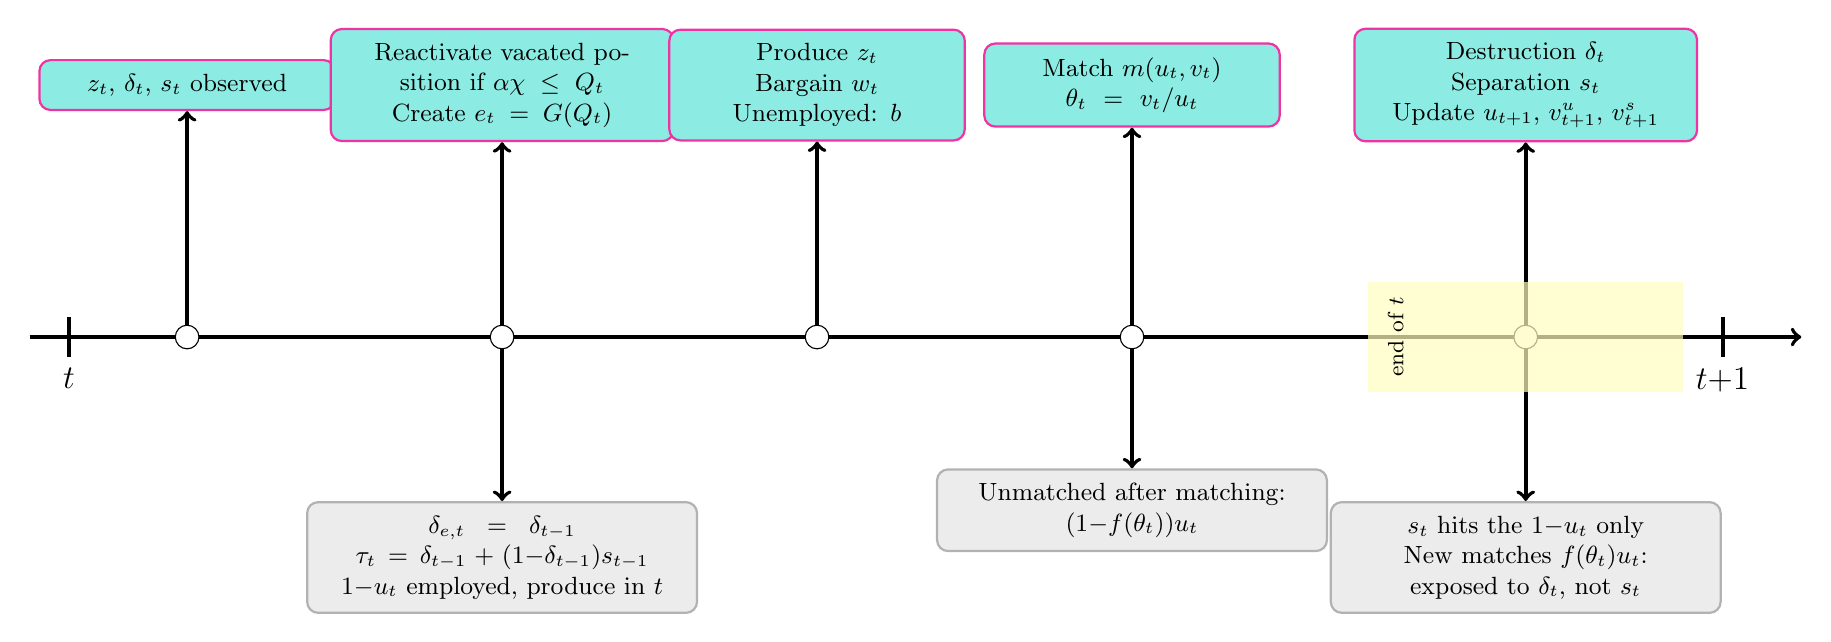
\begin{tikzpicture}[
	box/.style={draw=magenta!80, fill=turquoise!60, thick, rounded corners, align=center, font=\small, inner sep=5pt, text width=3.4cm},
	ebox/.style={draw=magenta!80, fill=turquoise!60, thick, rounded corners, align=center, font=\small, inner sep=5pt, text width=4.0cm},
	gbox/.style={draw=gray!60, fill=gray!15, thick, rounded corners, align=center, font=\small, inner sep=5pt, text width=4.6cm},
	dot/.style={circle, draw=black, fill=white, inner sep=0pt, minimum size=3mm},
	lw/.style={line width=0.5mm}]
	\draw[lw,->] (-0.5,0) -- (22,0);
	\draw[lw] (0, 0.25) -- (0,-0.25) node[below]{\large$t$};
	\draw[lw] (21,0.25) -- (21,-0.25) node[below]{\large$t{+}1$};
	\node[dot] (d1) at (1.5,0) {};
	\node[dot] (d2) at (5.5,0) {};
	\node[dot] (d3) at (9.5,0) {};
	\node[dot] (d4) at (13.5,0) {};
	\node[dot] (d5) at (18.5,0) {};
	\node[box] (B1) at (1.5, 3.2) {$z_t$, $\delta_t$, $s_t$ observed};
	\node[ebox] (B2) at (5.5, 3.2) {Reactivate vacated position if $\alpha\chi\leq Q_t$\\Create $e_t=G(Q_t)$};
	\node[box] (B3) at (9.5, 3.2) {Produce $z_t$\\Bargain $w_t$\\Unemployed: $b$};
	\node[box] (B4) at (13.5, 3.2) {Match $m(u_t,v_t)$\\$\theta_t=v_t/u_t$};
	\node[ebox] (B5) at (18.5, 3.2) {Destruction $\delta_t$\\Separation $s_t$\\Update $u_{t+1}$, $v^u_{t+1}$, $v^s_{t+1}$};
	\node[gbox] (C1) at (5.5, -2.8) {$\delta_{e,t}=\delta_{t-1}$\\$\tau_t=\delta_{t-1}+(1{-}\delta_{t-1})s_{t-1}$\\$1{-}u_t$ employed, produce in $t$};
	\node[gbox] (C2) at (13.5, -2.2) {Unmatched after matching:\\$(1{-}f(\theta_t))u_t$};
	\node[gbox] (C3) at (18.5, -2.8) {$s_t$ hits the $1{-}u_t$ only\\New matches $f(\theta_t)u_t$:\\exposed to $\delta_t$, not $s_t$};
	\foreach \d/\B in {d1/B1, d2/B2, d3/B3, d4/B4, d5/B5} \draw[lw,->] (\d) -- (\B);
	\draw[lw,->] (d2) -- (C1);
	\draw[lw,->] (d4) -- (C2);
	\draw[lw,->] (d5) -- (C3);
	\fill[yellow!25, opacity=0.7] (16.5,-0.7) rectangle (20.5,0.7);
	\node[font=\footnotesize, rotate=90] at (16.85,0) {end of $t$};
\end{tikzpicture}}
\caption{Timing within period $t$. Turquoise: decisions and events. Grey: implied stocks and rates. Yellow band: destruction and separation at the end of $t$.}\label{fig:timing}
\end{figure}

Unemployed workers and vacancies meet through a constant-returns matching function $m(u,v)$. With tightness $\theta_t=v_t/u_t$, the vacancy-filling rate is $q(\theta)=A\theta^{-\eta_L}$ and the job-finding rate is $f(\theta)=\theta q(\theta)$. A new match starts producing in the next period if its position survives.

A job position is a durable asset. Recruiters draw sunk costs of opening a position from the power law $G(x)=(x/x_m)^{\xi}$ on $[0,x_m]$ and open one whenever the cost is below the value of a vacancy $Q_t$, so $e_t=G(Q_t)$ new positions are created and
\begin{equation}\label{eq:Q}
Q_t = x_m e_t^{1/\xi}.
\end{equation}
The entry elasticity $\xi$ governs how elastic creation is, and vacancy free entry is the limit $\xi\to\infty$, in which $Q_t=x_m$. In addition, each hire costs $\kappa\ge0$. Destruction removes a product line and every position attached to it, filled or vacant, and a destroyed line is replaced by an identical one at no cost (clone replacement). Separation, in contrast, ends a match and leaves the position.

A position vacated by a separation at the end of $t-1$ draws a reactivation cost $\alpha\chi$ at $t$, independently across positions and periods, with cumulative distribution function
\begin{equation}
F_r(\chi) = (1-p_r) + p_r\chi^{\psi_r},\qquad \chi\in[0,1].
\end{equation}
With probability $1-p_r$ the cost is zero; otherwise it follows a power law with shape $\psi_r$ and upper bound $\alpha$. The position is reactivated if $\alpha\chi\le Q_t$ and retired otherwise, so the reactivation probability is
\begin{equation}\label{eq:Lambda_r}
\Lambda_{r,t} \equiv F_r\!\left(\frac{Q_t}{\alpha}\right) = 1-p_r+p_r\left(\frac{Q_t}{\alpha}\right)^{\psi_r},\qquad Q_t\le\alpha.
\end{equation}
The expected value of a vacated position, net of the cost paid, is
\begin{equation}\label{eq:Qrep}
Q_t^{rep}\equiv\E\big[\max\{Q_t-\alpha\chi,0\}\big] = Q_t\left[\Lambda_{r,t}-\frac{\psi_r}{1+\psi_r}\big(\Lambda_{r,t}-1+p_r\big)\right].
\end{equation}
Free positions keep all of $Q_t$, costly positions that are reactivated keep $Q_t$ net of their average cost, and retired positions keep nothing. With $p_r=0$, $\Lambda_{r,t}\equiv1$ and $Q_t^{rep}=Q_t$. Reactivation has its own cost distribution here; in the full model it shares the distribution of continuation costs.

A representative household of measure one has utility $\E_0\sum_t\beta^tC_t^{1-\sigma}/(1-\sigma)$. Each member supplies one unit of labor inelastically. Unemployed members enjoy a non-market flow $b$, which sets the outside option in bargaining but is not a market resource. The household holds shares in a mutual fund that owns every firm, in fixed supply, and trades a riskless bond in zero net supply.

\subsection{Equilibrium}\label{sec:equilibrium}

The household's first-order conditions price shares, $V_t=\E_t[m_{t+1}(V_{t+1}+D_{t+1})]$, and the riskless bond, $1=R^f_t\E_t[m_{t+1}]$, with the stochastic discount factor
\begin{equation}\label{eq:sdf}
m_{t+1} = \beta\left(\frac{C_{t+1}}{C_t}\right)^{-\sigma}.
\end{equation}
Firms act for their owners and value jobs and positions with $m_{t+1}$. Shares and bonds net out, so the household cannot change aggregate saving by trading. Instead, saving happens inside firms as investment in positions. The discount factor adjusts until households consume what firms do not invest. With $\sigma=0$, $m_{t+1}=\beta$, the risk-neutral case of \citet{gabrovski_2025}.

A filled position produces $z_t$, pays $w_t$ and, at the end of the period, survives as a match, becomes a vacated position, or is destroyed:
\begin{equation}\label{eq:value_matched}
J_t = z_t - w_t + \E_t m_{t+1}(1-\delta_t)\big[(1-s_t)J_{t+1}+s_tQ_{t+1}^{rep}\big].
\end{equation}
A vacancy is filled with probability $q(\theta_t)$, in which case the recruiter pays $\kappa$, and otherwise carries over. Since recruiters create positions until the marginal sunk cost equals the value of a vacancy, that value equals $Q_t$:
\begin{equation}\label{eq:value_unmatched}
Q_t = q(\theta_t)\big[\E_tm_{t+1}(1-\delta_t)J_{t+1}-\kappa\big] + \big(1-q(\theta_t)\big)\E_tm_{t+1}(1-\delta_t)Q_{t+1}.
\end{equation}
Define the flow value of a vacancy and the reposting shortfall,
\begin{align}
K_t &\equiv Q_t - \E_tm_{t+1}(1-\delta_t)Q_{t+1}, \label{eq:K}\\
\mathcal{R}_t &\equiv \E_tm_{t+1}(1-\delta_t)\big(Q_{t+1}-Q_{t+1}^{rep}\big). \label{eq:repost_shortfall}
\end{align}
$K_t$ is the cost of holding a position for a period: interest, the risk that destruction removes it, and capital losses when $Q$ falls. $\mathcal{R}_t$ is the value a separated position loses relative to costless reactivation, through retirement and the costs paid. Inserting \eqref{eq:K} into \eqref{eq:value_unmatched} places the average hiring cost on the left:
\begin{equation}\label{eq:average_hiring_cost}
\kappa+\frac{K_t}{q(\theta_t)} = \E_tm_{t+1}(1-\delta_t)\big(J_{t+1}-Q_{t+1}\big),
\end{equation}
and subtracting $Q_t$ from \eqref{eq:value_matched},
\begin{equation}\label{eq:value_surplus}
J_t-Q_t = z_t - w_t - K_t + (1-s_t)\left(\kappa+\frac{K_t}{q(\theta_t)}\right) - s_t\mathcal{R}_t.
\end{equation}

Wages are set by Nash bargaining. Workers' values are
\begin{align}
W_t &= w_t + \E_tm_{t+1}\big[(1-\tau_{t+1})W_{t+1}+\tau_{t+1}U_{t+1}\big],\\
U_t &= b + \E_tm_{t+1}\big[(1-\delta_t)f(\theta_t)W_{t+1}+\big(1-(1-\delta_t)f(\theta_t)\big)U_{t+1}\big],
\end{align}
where $\tau_{t+1}=\delta_t+(1-\delta_t)s_t$ is the separation rate between $t$ and $t+1$. Nash bargaining with worker share $\phi$, $(1-\phi)(W_t-U_t)=\phi(J_t-Q_t)$, gives
\begin{equation}\label{eq:wage}
w_t = \phi\big[z_t - K_t + \theta_t\big(K_t+q(\theta_t)\kappa\big) - s_t\mathcal{R}_t\big] + (1-\phi)b.
\end{equation}
The worker shares in the flow value saved and the hiring cost avoided, as in DMP with $K_t$ in place of a flow vacancy cost, and bears part of the reposting shortfall.

Substituting \eqref{eq:wage} into \eqref{eq:average_hiring_cost} and \eqref{eq:value_surplus} gives the job creation condition:
\begin{multline}\label{eq:jcc}
\kappa+\frac{K_t}{q(\theta_t)} = \E_t m_{t+1}(1-\delta_t)\Big[(1-\phi)(z_{t+1}-K_{t+1}-b) - \phi\theta_{t+1}K_{t+1} - \phi f(\theta_{t+1})\kappa \\
+ (1-s_{t+1})\left(\kappa+\frac{K_{t+1}}{q(\theta_{t+1})}\right) - (1-\phi)s_{t+1}\mathcal{R}_{t+1}\Big].
\end{multline}

Unemployment and the two inherited vacancy stocks evolve as
\begin{align}
u_{t+1} &= u_t - (1-\delta_t)f(\theta_t)u_t + \tau_{t+1}(1-u_t), \label{eq:u_lom}\\
v^u_{t+1} &= (1-\delta_t)\big(1-q(\theta_t)\big)v_t, \label{eq:vu_lom}\\
v^s_{t+1} &= (1-\delta_t)s_t(1-u_t), \label{eq:vs_lom}
\end{align}
where $v^u_{t+1}$ is the stock of vacancies that went unmatched in $t$ and survived destruction, and $v^s_{t+1}$ is the stock of positions vacated by separation at the end of $t$, whose reactivation is decided at the start of $t+1$. Vacancies in period $t$ then combine the two inherited stocks with new positions,
\begin{equation}\label{eq:v_lom}
v_t = v^u_t + \Lambda_{r,t}v^s_t + e_t.
\end{equation}
Destruction reduces both inherited stocks, so a destruction shock removes vacancies as well as jobs. Unmatched vacancies are posted again with certainty, whereas vacated positions are posted only if reactivated, with probability $\Lambda_{r,t}=F_r(Q_t/\alpha)$. Because $Q_t$ responds to the shocks of period $t$, the number of inherited vacancies actually posted, $v^u_t+\Lambda_{r,t}v^s_t$, is not known at the end of $t-1$; only the two stocks are, and they must be carried as separate states. With costless reactivation, $\Lambda_{r,t}=1$ and the two stocks collapse into a single predetermined stock of vacancies, $v^u_t+v^s_t$, as in \citet{gabrovski_2025}; the same holds under vacancy free entry, where $Q_t$ and hence $\Lambda_{r,t}$ are constant. Finally, creation $e_t=G(Q_t)$ is non-negative by construction, so positions are never scrapped other than through destruction or retirement.

Output is $z_t(1-u_t)$. Spending on creation and hiring is $X_t = \frac{\xi}{1+\xi}Q_te_t + \kappa q(\theta_t)v_t$, and spending on reactivation is $X_t^r = v^s_t\big(Q_t\Lambda_{r,t}-Q_t^{rep}\big)$. Consumption is
\begin{equation}\label{eq:resources}
C_t = z_t(1-u_t) - X_t - X_t^r.
\end{equation}

\begin{definition}
Given initial stocks and the processes \eqref{eq:ar1_z}--\eqref{eq:ar1_s}, an equilibrium is a stochastic sequence $\{\theta_t, e_t, C_t, u_{t+1}, v^u_{t+1}, v^s_{t+1}\}$ with $Q_t$, $\Lambda_{r,t}$ and $Q_t^{rep}$ given by \eqref{eq:Q}--\eqref{eq:Qrep}, $m_{t+1}$ by \eqref{eq:sdf}, and $K_t$ and $\mathcal{R}_t$ by \eqref{eq:K}--\eqref{eq:repost_shortfall}, such that job creation \eqref{eq:jcc}, the laws of motion \eqref{eq:u_lom}--\eqref{eq:v_lom} and the resource constraint \eqref{eq:resources} hold for all $t$.
\end{definition}

The jump variables are $\theta_t$, $e_t$ and $C_t$; the states are $u_t$, $v^u_t$, $v^s_t$ and the shocks. Table~\ref{tab:dmp} compares the model with DMP.

\begin{table}[H]
\centering
\caption{The model and DMP, term by term}\label{tab:dmp}
\small
\begin{tabular}{p{3.2cm}p{4.5cm}p{6.8cm}}
\toprule
 & DMP & This model \\
\midrule
Vacancy cost & flow cost & flow value $K_t$: interest, depreciation through $\delta_t$, capital losses when creation falls \\
Discounting & $\beta$ & $m_{t+1}=\beta(C_{t+1}/C_t)^{-\sigma}$ \\
Separation & the firm posts again & the shortfall $s_t\mathcal{R}_t$ acts like a firing cost \\
Vacancies & jump variable & inherited stocks $v^u_t$, $v^s_t$ plus creation $e_t$ \\
Destruction & not separate from separation & removes jobs and the vacancies attached \\
\bottomrule
\end{tabular}
\end{table}

\subsection{Special cases}

\begin{remark}[Nesting]\label{rem:nesting}
With costless reactivation ($p_r=0$), $\Lambda_{r,t}\equiv1$, $Q_t^{rep}=Q_t$ and $\mathcal{R}_t=0$: separations remove no positions, and with $\kappa=0$ and $\sigma=0$ the model is \citet{gabrovski_2025} with aggregate shocks. If in addition $s_t\equiv0$, every separation is destruction and the model has the structure of \citet{coles_2018}.
\end{remark}

\begin{lemma}[Tightness under vacancy free entry]\label{lem:theta}
Let $\sigma=0$ and $\xi\to\infty$. Then $Q_t=x_m$, $K_t=x_m[1-\beta(1-\delta_t)]$ and $\mathcal{R}_t=\beta(1-\delta_t)\big(x_m-Q^{rep}(x_m)\big)$ depend on the current shock alone, and \eqref{eq:jcc} determines $\theta_t$ as a function of current and expected future shocks only. Tightness does not load on unemployment or the vacancy stocks.
\end{lemma}
\begin{proof}
In the limit $Q_t=x_m$ for every $e_t$, so $\Lambda_{r,t}$ and $Q_t^{rep}$ are constant and $K_t$ and $\mathcal{R}_t$ follow from \eqref{eq:K}--\eqref{eq:repost_shortfall} with $m_{t+1}=\beta$. Equation \eqref{eq:jcc} then involves only $\theta_t$, $\theta_{t+1}$ and the shocks, so its solution does not depend on the stocks. Creation $e_t$ adjusts through \eqref{eq:v_lom} to deliver $\theta_t$.
\end{proof}
% Checked numerically: ags_run_solution.txt, "Check (σ = 0)".
In this limit, separations still move tightness through two terms of \eqref{eq:jcc}: the continuation value, as in DMP, and the shortfall. Destruction moves it through the flow value $K_t$. With $\sigma>0$ the lemma fails, because the discount factor depends on consumption and consumption on the stocks.

\subsection{Steady state}

In steady state $m=\beta=1/(1+r)$ whatever $\sigma$, so $\sigma$ affects only the dynamics. Given $\theta$: $q=A\theta^{-\eta_L}$, $f=\theta q$, $u=\tau/(\tau+(1-\bar\delta)f)$ and $v=\theta u$, with $\tau=\bar\delta+(1-\bar\delta)\bar s$. Creation replaces the positions destroyed and those retired,
\begin{equation}
e = \bar\delta(v+1-u) + (1-\bar\delta)(1-\Lambda_r)\bar s(1-u),\qquad Q = x_me^{1/\xi},
\end{equation}
which has a unique solution in $Q$ because a higher $Q$ raises reactivation and lowers the creation needed. The flow value and the shortfall are
\begin{equation}
K = Q\,\frac{r+\bar\delta}{1+r},\qquad \mathcal{R} = \frac{(1-\bar\delta)\big(Q-Q^{rep}\big)}{1+r}.
\end{equation}
Job creation reads
\begin{equation}\label{eq:jc_ss}
(1-\phi)(\bar z - K - b - \bar s\mathcal{R}) - \phi\theta(K+q\kappa) = \frac{r+\tau}{1-\bar\delta}\left(\kappa+\frac{K}{q}\right):
\end{equation}
the recruiter's share of the flow surplus covers the hiring cost, annuitized over the expected life of a match. As $\theta$ rises the left side falls and the right side rises, so the steady state is unique.

% =============================================================================
\section{Calibration and estimation}\label{sec:calibration}
% =============================================================================

We proceed in three steps. The long-run parameters are set so that the steady state reproduces average flows in the data. The shock processes are calibrated in advance from the SVAR. Five parameters that govern propagation are then estimated by matching the model's responses to productivity and separation shocks to those in the data, while the responses to destruction are held out as a test.

\subsection{Long-run targets}

We calibrate the model by running the steady state in reverse. Because every unknown then enters linearly, the calibration is in closed form for any value of the estimated parameters. The levels come from the same series as the SVAR, averaged over 1992Q3--2019Q4 (Table~\ref{tab:targets}). The BED death rate is 0.225 percent a month. The CPS gross flows give a separation rate into unemployment of 1.34 percent a month and a job-finding rate of 0.252 a month. Destruction therefore accounts for 17 percent of separations into unemployment, as in Section~\ref{sec:beyond_ck}.
% ags_steady_state.jl AGS_TARGETS (D19): dest_ann 0.026665 = 12 x 0.0022497, sep 0.013380, f 0.2524; shock_calibration.txt §1 (delta/tau = 0.1681)

\begin{table}[H]
\centering
\caption{Targets and the parameters they pin down}\label{tab:targets}
\small
\begin{tabular}{p{5.2cm}p{2.2cm}p{5.2cm}p{2.2cm}}
\toprule
Target & Value & Source & Pins \\
\midrule
Destruction rate & 0.225\% a month & BED Deaths, 1992Q3--2019Q4 & $\bar\delta$ \\
Separation rate into unemployment & 1.34\% a month & CPS gross flows, E$\to$U, 1992Q3--2019Q4 & $\bar s$ via $\tau=\delta+(1-\delta)s$ \\
Job-finding rate & 0.252 a month & CPS gross flows, U$\to$E, 1992Q3--2019Q4 & $A$, $\theta$ \\
Vacancy-filling rate & 0.80 a month & JOLTS & $\theta$ \\
Matching elasticity & 0.6 & \citet{petrongolo_2001} & $\eta_L$ \\
Interest rate & 4\% a year & & $\beta$ \\
Wage & 1 & normalization & $\phi$ \\
Recruiting costs / output & 1.5\% & & $Q$, then $x_m$ \\
Costly share, shape & 0.99, 1 & & $p_r$, $\psi_r$ \\
\midrule
\multicolumn{4}{l}{Estimated (Section~\ref{sec:estimation}): $b/w$, the sunk share of the cost of a hire $x_v$, the creation elasticity $\xi$,} \\
\multicolumn{4}{l}{the reactivation rate $\bar\Lambda_r$, and risk aversion $\sigma$.} \\
\bottomrule
\end{tabular}
\end{table}
% TODO(MS): source for the recruiting-cost share X/Y (Draft.tex tab:calib_targets).

The job-finding and filling rates, divided by $1-\delta$ to condition on survival, give $\theta$, $u$, $v$ and $A$ directly. With $\bar\Lambda_r$ given, creation $e$ is explicit. Per unit of $Q$, the flow value is $K/Q=(r+\bar\delta)/(1+r)$, the hiring cost is fixed relative to it by the sunk share, and the reactivation shortfall is
\begin{equation}
\frac{\mathcal{R}}{Q} = \frac{1-\bar\delta}{1+r}\left[(1-\bar\Lambda_r) + \frac{\psi_r}{1+\psi_r}(\bar\Lambda_r-1+p_r)\right].
\end{equation}
The flow surplus $\bar z-w$ and recruiting costs $X$ are then both linear in $Q$, so the target for $X/Y$ pins $Q$ without root-finding. Job creation \eqref{eq:jc_ss} gives $\bar z$, the wage equation gives $\phi$, and \eqref{eq:Q} gives $x_m=Qe^{-1/\xi}$. The scale $\alpha$ follows from $\bar\Lambda_r$. Solving forward from the calibrated parameters recovers every target to machine precision. % ags_steady_state_checks.txt

Table~\ref{tab:ss} reports the steady state at the estimates of Section~\ref{sec:estimation}. The targets fix $u$, $\theta$ and $v$, which are therefore the same under both filters. The estimated parameters move the value of a position $Q$, the hiring cost $\kappa$, average productivity $\bar z$ and the bargaining power $\phi$, which the wage normalization implies rather than sets.

\begin{table}[H]
\centering
\caption{Steady state at the estimates}\label{tab:ss}
\small
\begin{tabular}{lcc}
\toprule
 & HP estimates & Hamilton estimates \\
\midrule
$u$ & 0.0503 & 0.0503 \\
$\theta$ & 0.3155 & 0.3155 \\
$v$ & 0.0159 & 0.0159 \\
$\bar\Lambda_r$ & 0.03 & 0.03 \\
$Q$ & 2.4868 & 4.5603 \\
$\kappa$ & 0.2735 & 0.1673 \\
$\bar z$ & 1.0456 & 1.0780 \\
$\phi$ & 0.2769 & 0.5694 \\
\bottomrule
\end{tabular}
\end{table}
% ags_estimate_report_hp.txt and ags_estimate_report_ham.txt §1

\subsection{Shock processes}\label{sec:shocks}

Each shock follows an AR(1) in logs at a monthly frequency. We calibrate the three processes in advance from SVAR~A itself, the system through which we compare model and data, separately for each filter. The persistence of a process is the own-lag coefficient of its equation, which conditions on the lagged values of every variable in the system. Its size is the standard deviation of the structural shock's impact on its own series, the diagonal of the Cholesky factor, which nets out the shocks ordered before it.
% part6e_window_processes.py; shock_calibration_window.csv; decisions.md D20

The alternative, a univariate AR(1) for each series, would attribute to a shock's process persistence that the SVAR assigns to other shocks. The difference matters for separations. Measured with gross flows, the separation rate is strongly countercyclical. Its univariate quarterly persistence is 0.73, whereas its own-lag coefficient in SVAR~A is 0.15. Most of the persistence of the separation rate thus comes from the lagged state of the economy, not from its own past. The model has no channel through which productivity or labor-market conditions move separations, so a univariate process would give the exogenous separation shock persistence that in the data belongs to the responses to other shocks. With univariate processes, the estimation below fits the separation responses badly under both filters, with the parameters at the edges of their ranges.
% shock_calibration.txt (s: rho_Q 0.7278, 1951Q1-2019Q4 spliced); shock_calibration_window.csv hp_rho_Q (s 0.1455); findings.md "AGS estimated with gross flows" (univariate: J_s 320 HP, 411 Hamilton)

Our approach generalizes that of \citet{coles_2018}. They match independent AR(1) processes for productivity and separations to the quarterly autocorrelations of each series and allow the two innovations to be correlated. We condition persistence on the full system and orthogonalize the innovations, as the SVAR does. One consequence is that the part of the separation rate that responds to productivity within the quarter is not in the exogenous separation process. The model would have to produce that part itself, and it has no mechanism to do so.
% CK p. 124 and Table 2: independent AR(1)s, rho_p 0.965, rho_delta 0.875 (monthly), innovation correlation -0.63, matched to quarterly first-order autocorrelations and the cross-correlation in Shimer (2005) data.

Plugging the quarterly estimates directly into monthly processes would understate the data's quarterly statistics, since time averaging and the filter cut the standard deviation of the cycle by 21 to 29 percent.
% shock_calibration.txt §7
We therefore choose each monthly $(\rho,\sigma)$ so that simulated data reproduce the quarterly targets (500 replications). The simulated data are averaged to quarters, filtered over each series' own span as the data are (productivity from 1951, separations from 1990, destruction from 1992), and fitted on SVAR~A's window.\footnote{In the model the three processes are exogenous and mutually independent, so, up to time aggregation, a univariate fit on simulated data estimates the same object as the own-lag coefficient of the SVAR. Appendix~\ref{app:validation} checks the own responses through the SVAR directly.} Under the Hamilton filter, no stationary monthly AR(1) attains the data's quarterly persistence of productivity, and we set its persistence at 0.999. Table~\ref{tab:shocks} gives the processes.
% part6b match_process (Step 4b); part6e_window_processes.py

\begin{table}[H]
\centering
\caption{Shock processes: quarterly targets from SVAR~A and matched monthly AR(1) processes in logs}\label{tab:shocks}
\small
\setlength{\tabcolsep}{4pt}
\begin{tabular}{lccccc@{\hspace{0.5cm}}ccccc}
\toprule
 & \multicolumn{5}{c}{HP, 1992Q3--2019Q4} & \multicolumn{5}{c}{Hamilton, 1995Q2--2019Q4} \\
 & \multicolumn{2}{c}{Target} & \multicolumn{2}{c}{Monthly} & Univariate & \multicolumn{2}{c}{Target} & \multicolumn{2}{c}{Monthly} & Univariate \\
 & $\rho_Q$ & $\sigma_Q$ & $\rho$ & $\sigma$ & $\rho$ & $\rho_Q$ & $\sigma_Q$ & $\rho$ & $\sigma$ & $\rho$ \\
\midrule
$z$ & 0.6350 & 0.0055 & 0.8830 & 0.0044 & 0.9409 & 0.9120 & 0.0092 & 0.9990 & 0.0044 & 0.9990 \\
$\delta$ & 0.1696 & 0.0538 & 0.4991 & 0.0648 & 0.5319 & 0.6864 & 0.0590 & 0.8560 & 0.0478 & 0.8923 \\
$s$ & 0.1455 & 0.0387 & 0.4585 & 0.0482 & 0.9606 & 0.3355 & 0.0638 & 0.5860 & 0.0693 & 0.9943 \\
\bottomrule
\multicolumn{11}{p{0.95\linewidth}}{\footnotesize \textit{Notes.} Target: own-lag coefficient ($\rho_Q$) and own impact of the one-standard-deviation structural shock ($\sigma_Q$) in SVAR~A. Monthly: the matched process used. Univariate: the monthly persistence matched to each series' univariate AR(1) instead, for comparison. The Hamilton process for $z$ is at the bound and does not attain its target.}
\end{tabular}
\end{table}
% shock_calibration_window.csv: <f>_rho_Q, <f>_sigma_Q, <f>_rho_m, <f>_sigma_m, <f>_uni_rho_m

The new processes are much less persistent for separations: a monthly persistence of 0.46 instead of 0.96 under HP. For productivity and destruction they change little.

\subsection{Estimation}\label{sec:estimation}

We estimate five parameters by indirect inference \citep{gourieroux_1993}, matching impulse responses as in \citet{christiano_2005}. The auxiliary model is SVAR~A with the job-finding rate ordered last, $(z,s,\delta,u,v,f)$, with one lag selected by the BIC under both filters. Adding $f$ disciplines the outflow channel, which carries most of the destruction response in the data (Section~\ref{sec:facts}). The moments are the responses of $u$, $v$ and $f$ to one-standard-deviation productivity and separation shocks at horizons 0 to 12, which gives 78 moments. Their data values and standard deviations come from the SVAR and a 1,000-draw residual bootstrap.
% q3_estimation_targets.py; estimation_targets.csv (BIC p = 1, HP T = 110, Hamilton T = 99)

For a given parameter vector $\vartheta$, we calibrate the steady state as above, solve the model to first order, and simulate it monthly. We draw $R$ windows of data length, average each to quarters, filter it as the data are, and estimate the same SVAR on it. The model's moments $\bar m(\vartheta)$ are the mean responses over the windows. The estimator minimizes
\begin{equation}\label{eq:loss}
J(\vartheta)=\sum_{k=1}^{78}\left(\frac{\bar m_k(\vartheta)-d_k}{\text{sd}_k}\right)^2,
\end{equation}
where $d_k$ is the data's response and $\text{sd}_k$ its bootstrap standard deviation. A model whose responses lie within one standard deviation of the data's on average has $J$ of about 78, or 39 for each shock. As in \citet{christiano_2005}, the weights use only the variances. The simulations reuse the same random numbers at every $\vartheta$, so the objective is a deterministic function of the parameters. We search over a coarse grid of $\sigma$ and $\bar\Lambda_r$ with $R=50$, start a Nelder--Mead search from the two best points, and evaluate the best point with $R=200$.
% ags_estimate.jl (AGS_MODE = search, final); decisions.md D18

The estimated parameters are those that govern propagation and that the long-run targets leave free. The reactivation rate $\bar\Lambda_r\in[0.03,0.99]$ sets how many positions separations retire. The creation elasticity $\xi\in[0.25,10]$ sets how fast lost positions are rebuilt. The sunk share of the cost of a hire $x_v\in[0.05,0.9]$ splits that cost between the position and the hire. The ratio $b/w\in[0.5,0.97]$ sets the size of the surplus and therefore the elasticity of job creation to productivity. Risk aversion $\sigma\in[0,4]$ sets how strongly the household's discount factor moves with consumption, which matters because households own the firms and value positions with that factor. We fix the matching elasticity at 0.6 \citep{petrongolo_2001}.

The responses to destruction, another 39 moments, are held out. Once the responses to separations have pinned down the reactivation rate, the response to destruction has no free parameter left in the positions channel, so it is a test of the model's propagation. The statistic $J_\delta$ is the distance \eqref{eq:loss} over these moments. Its distribution under the model comes from the simulations: for each of the 200 windows, we compute the same distance between that window's responses and the model's mean. The $p$-value is the share of windows farther from the mean than the data.
% ags_estimate.jl final(): Jw, pval

% =============================================================================
\section{The estimated model against the SVAR}\label{sec:results}
% =============================================================================

We solve the model by first-order perturbation in logs; a pruned second-order solution changes the moments negligibly.
% ags_order_check.txt
% TODO(MS): ags_order_check.txt predates D19/D20; rerun at the estimates.
Table~\ref{tab:estimates} reports the estimates and the fit, and Table~\ref{tab:irf_compare} the responses under the HP filter. The Hamilton responses are in Appendix~\ref{app:filters}.

\begin{table}[H]
\centering
\caption{Estimates and fit}\label{tab:estimates}
\small
\begin{tabular}{lcc}
\toprule
 & HP & Hamilton \\
\midrule
Risk aversion $\sigma$ & 4.00$^{b}$ & 0.00$^{b}$ \\
Reactivation rate $\bar\Lambda_r$ & 0.03$^{b}$ & 0.03$^{b}$ \\
Creation elasticity $\xi$ & 0.59 & 0.30 \\
Sunk share $x_v$ & 0.06 & 0.16 \\
$b/w$ & 0.97$^{b}$ & 0.93 \\
Implied bargaining power $\phi$ & 0.28 & 0.57 \\
\midrule
$J_z$ (39 moments; $u$, $v$, $f$) & 180.1 (87.0, 45.9, 47.2) & 73.6 (52.1, 11.5, 9.9) \\
$J_s$ (39 moments; $u$, $v$, $f$) & 44.8 (13.1, 22.6, 9.2) & 83.6 (26.5, 35.3, 21.8) \\
\midrule
Test: $J_\delta$ (39 moments; $u$, $v$, $f$) & 161.4 (58.6, 52.0, 50.8) & 18.2 (9.2, 7.4, 1.5) \\
Simulated $J_\delta$: median, 95th, 99th percentile & 2.4, 12.4, 24.7 & 19.2, 72.4, 102.3 \\
$p$-value & 0.000 & 0.520 \\
\bottomrule
\multicolumn{3}{p{0.75\linewidth}}{\footnotesize \textit{Notes.} $^{b}$ at a bound of the search. $R=200$ simulated windows. Data: HP, 1992Q3--2019Q4 ($T=110$); Hamilton, 1995Q2--2019Q4 ($T=99$).}
\end{tabular}
\end{table}
% ags_estimate_report_hp.txt and ags_estimate_report_ham.txt §1-2; ags_estimate_final_<filter>.csv

\begin{table}[H]
\centering
\caption{Responses through the SVAR under the HP filter: estimated model and data (one SD; log points $\times$ 100)}\label{tab:irf_compare}
\footnotesize
\setlength{\tabcolsep}{3.5pt}
\begin{tabular}{llcccc@{\hspace{0.5cm}}cccc}
\toprule
 & & \multicolumn{4}{c}{Model} & \multicolumn{4}{c}{Data} \\
Shock & Response & $h=0$ & Peak (quarter) & $h=8$ & Sum, 0--12 & $h=0$ & Peak (quarter) & $h=8$ & Sum, 0--12 \\
\midrule
$z$ & $u$ & $-0.14$ & $-1.16$ (3) & $-0.10$ & $-5.2$ & $-0.97$ & $-2.74$ (4) & $-1.81$ & $-23.1$ \\
 & $v$ & $+1.85$ & $+2.70$ (1) & $-0.11$ & $+11.1$ & $+0.81$ & $+2.97$ (3) & $+1.44$ & $+21.8$ \\
 & $f$ & $+0.79$ & $+1.36$ (2) & $-0.00$ & $+6.5$ & $+0.49$ & $+1.80$ (4) & $+1.24$ & $+15.2$ \\
$s$ & $u$ & $+0.75$ & $+1.88$ (1) & $-0.11$ & $+5.1$ & $+1.46$ & $+1.46$ (0) & $-0.07$ & $+5.5$ \\
 & $v$ & $+0.16$ & $-1.86$ (2) & $+0.30$ & $-3.4$ & $-1.04$ & $-1.19$ (1) & $+0.26$ & $-2.7$ \\
 & $f$ & $-0.24$ & $-1.25$ (2) & $+0.16$ & $-3.4$ & $-0.05$ & $-0.79$ (2) & $+0.02$ & $-2.6$ \\
$\delta$ & $u$ & $+0.25$ & $+0.50$ (1) & $-0.04$ & $+1.3$ & $+0.48$ & $+1.58$ (3) & $+0.75$ & $+11.8$ \\
 & $v$ & $+0.02$ & $-0.47$ (2) & $+0.10$ & $-0.7$ & $-0.33$ & $-1.87$ (2) & $-0.51$ & $-11.0$ \\
 & $f$ & $-0.11$ & $-0.33$ (1) & $+0.06$ & $-0.8$ & $-0.30$ & $-1.02$ (3) & $-0.53$ & $-7.6$ \\
\bottomrule
\multicolumn{10}{p{0.95\linewidth}}{\footnotesize \textit{Notes.} SVAR $(z,s,\delta,u,v,f)$, one lag. Model: mean over 200 simulated windows of 110 quarters at the HP estimates. The responses to $z$ and $s$ are estimated; those to $\delta$ are the test.}
\end{tabular}
\end{table}
% ags_estimate_report_hp.txt §3; ags_estimate_irf_hp.csv
% TODO(MS): figure of the model and data responses with bands (replaces the pre-D19 q3_model_svar.png).

\subsection{Separations}

The estimated model fits the responses to separations. Under the HP filter $J_s$ is 45, close to the value of 39 that one standard deviation per moment would give. Summed over three years, unemployment rises by 5.1 points in the model against 5.5 in the data, although the model's response peaks a quarter later. The one systematic miss is the timing of vacancies. On impact they rise slightly in the model (+0.16) but fall in the data ($-1.04$), and the model's trough comes a quarter later and is deeper, at $-1.86$ after two quarters against the data's $-1.19$ after one.
% ags_estimate_report_hp.txt §2-3

The reactivation rate is estimated at the bottom of its range, 0.03, under both filters: separations retire nearly every position they vacate, which is the assumption of \citet{coles_2018} for every separation. The responses to separations identify this rate sharply. With the other parameters at their estimates, raising $\bar\Lambda_r$ from 0.03 to 0.95 raises $J_s$ from 48 to 193 under HP and from 99 to 457 under Hamilton (Table~\ref{tab:reactivation}). A high reactivation rate replaces vacated positions quickly, and the rise in unemployment after a separation shock is then too small and too brief.
% ags_estimate_report_<filter>.txt §5 (R = 50)

\subsection{Productivity}

The model fails on productivity, and the failure is one of persistence. Under HP the model's productivity process reproduces the data's own response of productivity through the SVAR (Appendix~\ref{app:validation}), so the impulse is right. Yet unemployment falls by at most 1.16 points in the model against 2.74 in the data. The response is near zero after two years in the model, whereas in the data it is still two-thirds of its peak. Summed over three years the model delivers less than a quarter of the data's response, and the responses of vacancies and job finding show the same pattern. In the data, the response of productivity itself is short-lived, so the long response of unemployment is propagation that the model lacks. Under the Hamilton filter the productivity process is far more persistent and the fit improves ($J_z=74$), but the model still delivers about two-fifths of the data's response.
% ags_estimate_report_hp.txt §3-4 (z own: model 0.52, 0.35, 0.17 vs data 0.54, 0.32, 0.18; u sum -5.2 vs -23.1; h8 -1.81/-2.74 = 0.66); ags_estimate_report_ham.txt §3 (sum -19.8 vs -48.7)

The misfit to productivity drives the other HP estimates. Risk aversion and $b/w$ sit at the upper bounds of their ranges, the direction that strengthens the response to productivity; a high $b/w$ leaves a small surplus, as in \citet{hagedorn_2008}. Moving $\sigma$ from 0 to 4 lowers $J_z$ from 259 to 185 under HP and leaves the fit to separations unchanged; under Hamilton, $J$ barely moves with $\sigma$, which is estimated at zero. Risk aversion is thus weakly identified. Moving it by a tenth of its range changes the 78 moments by 0.65 data standard deviations (the root of the sum of squares), against 19 for the creation elasticity. We therefore do not report standard errors, which are not meaningful at the bounds, and show profiles instead.
% ags_estimate_report_<filter>.txt §5-6 (sensitivity: sigma 0.65 HP / 0.26 Ham; xi 19.05 / 32.66)

\subsection{Destruction: the test}

Under the HP filter the model fails the test decisively. $J_\delta$ is 161, whereas the 99th percentile of its simulated distribution is 25 and no simulated window is as far from the model as the data are. Unemployment rises by 0.25 points on impact in the model against 0.48 in the data. The model's response peaks after one quarter at 0.50, against 1.58 after three quarters in the data, and summed over three years it is 1.3 points against 11.8. Vacancies and job finding fall to between a quarter and a third of the data's troughs.
% ags_estimate_report_hp.txt §2-3

Under the Hamilton filter the test does not reject ($p=0.52$). This reflects the low power of the test on that sample rather than a good fit. The Hamilton responses are much less precise, so the 95th percentile of the simulated $J_\delta$ is 72, against 12 under HP. The model's response of unemployment again reaches about half the data's peak, at 0.98 after two quarters against 2.05 after five, and summed over three years it is 7.0 points against 18.1 (Appendix~\ref{app:filters}).
% ags_estimate_report_ham.txt §2-3

% =============================================================================
\section{The puzzle}\label{sec:puzzle}
% =============================================================================

After a destruction shock, the estimated model's response of unemployment is about half the data's on impact and is gone within two years, whereas the data's keeps building for three quarters. Productivity shows a similar failure. Both gaps are thus mainly about propagation, not about the impulse: the model reproduces the data's own responses of productivity and, under Hamilton, of destruction (Appendix~\ref{app:validation}).

If persistence came from lost positions, lowering the reactivation rate would supply it. As Table~\ref{tab:reactivation} shows, it does so for separations but not for destruction. At the HP estimates, as $\bar\Lambda_r$ falls from 0.95 to 0.03, the model's cumulative response of unemployment to a separation shock rises from 4.1 to 10.5 points, and $J_s$ falls from 193 to 48. The response to destruction, however, barely changes: it peaks after one quarter at 0.37 to 0.38 points, and $J_\delta$ stays between 161 and 163. Under Hamilton the pattern is the same. The reason is simple. Reactivation applies only to positions vacated by separations, whereas a destroyed position is gone whatever the reactivation rate.
% ags_estimate_report_hp.txt and ags_estimate_report_ham.txt §5

\begin{table}[H]
\centering
\caption{The estimated model across reactivation rates (other parameters at the estimates)}\label{tab:reactivation}
\small
\begin{tabular}{lccccccc}
\toprule
 & & \multicolumn{2}{c}{Fit through the SVAR} & \multicolumn{2}{c}{True $\delta\to u$} & \multicolumn{2}{c}{True $s\to u$} \\
$\bar\Lambda_r$ & $\phi$ & $J_s$ & $J_\delta$ & peak (q) & sum, q0--12 & peak (q) & sum, q0--12 \\
\midrule
\multicolumn{8}{l}{\textit{HP estimates}} \\
0.03 & 0.277 & 47.7 & 161.0 & 0.37 (1) & 3.2 & 1.24 (1) & 10.5 \\
0.10 & 0.267 & 48.3 & 161.3 & 0.37 (1) & 3.2 & 1.19 (1) & 10.0 \\
0.25 & 0.246 & 56.6 & 162.1 & 0.37 (1) & 3.3 & 1.09 (1) & 8.9 \\
0.50 & 0.208 & 89.6 & 162.8 & 0.37 (1) & 3.4 & 0.93 (1) & 7.1 \\
0.75 & 0.166 & 142.5 & 162.8 & 0.37 (1) & 3.6 & 0.78 (1) & 5.4 \\
0.95 & 0.129 & 193.4 & 162.0 & 0.38 (1) & 3.7 & 0.69 (0) & 4.1 \\
\multicolumn{8}{l}{\textit{Hamilton estimates}} \\
0.03 & 0.569 & 98.9 & 15.5 & 0.66 (4) & 6.8 & 2.20 (1) & 18.6 \\
0.10 & 0.556 & 103.4 & 15.7 & 0.66 (4) & 6.7 & 2.11 (1) & 17.2 \\
0.25 & 0.524 & 129.9 & 16.3 & 0.65 (4) & 6.6 & 1.92 (1) & 14.5 \\
0.50 & 0.459 & 211.7 & 17.2 & 0.65 (4) & 6.6 & 1.61 (1) & 10.4 \\
0.75 & 0.373 & 334.1 & 18.1 & 0.66 (4) & 6.8 & 1.31 (1) & 6.6 \\
0.95 & 0.282 & 456.7 & 17.5 & 0.68 (4) & 7.1 & 1.07 (1) & 3.5 \\
\bottomrule
\multicolumn{8}{p{0.9\linewidth}}{\footnotesize \textit{Notes.} $J_s$ and $J_\delta$: distance \eqref{eq:loss} through the SVAR, $R=50$ windows. True responses: one-SD shocks, quarterly averages of the monthly responses, log points $\times$ 100.}
\end{tabular}
\end{table}
% ags_estimate_report_hp.txt and ags_estimate_report_ham.txt §5

This is an overidentifying test. The separation responses identify the reactivation rate, and once it is set, the destruction response has no free parameter left in the positions channel; the model fails the test at any reactivation rate under HP. Unconditional persistence, the moment \citet{coles_2018} match, cannot make this distinction, because a low reactivation rate combined with persistent separations reproduces it. The conditional responses can.

The puzzle, then, is the following. A short-lived rise in establishment deaths, which removes few positions, depresses job finding for about two years, while larger losses of positions through separations do not. Something lost only when an establishment dies, or something that a death sets in motion, keeps job creation low. Within the model, neither the number of positions lost nor how fast they are re-created supplies it.

% =============================================================================
\section{Conclusion}\label{sec:conclusion}
% =============================================================================

% TODO: written after the puzzle's resolution or framing is settled (decisions.md D16).

\appendix

\section{Results under the Hamilton filter}\label{app:filters}

Under the filter of \citet{hamilton_2018} ($h=8$, $p=4$) the window starts in 1995Q2 ($T=99$), and the shock processes are more persistent (Table~\ref{tab:shocks}). Table~\ref{tab:irf_ham} reports the responses at the Hamilton estimates.

\begin{table}[H]
\centering
\caption{Responses through the SVAR under the Hamilton filter: estimated model and data (one SD; log points $\times$ 100)}\label{tab:irf_ham}
\footnotesize
\setlength{\tabcolsep}{3.5pt}
\begin{tabular}{llcccc@{\hspace{0.5cm}}cccc}
\toprule
 & & \multicolumn{4}{c}{Model} & \multicolumn{4}{c}{Data} \\
Shock & Response & $h=0$ & Peak (quarter) & $h=8$ & Sum, 0--12 & $h=0$ & Peak (quarter) & $h=8$ & Sum, 0--12 \\
\midrule
$z$ & $u$ & $+0.20$ & $-2.22$ (5) & $-1.82$ & $-19.8$ & $-2.20$ & $-4.36$ (6) & $-4.26$ & $-48.7$ \\
 & $v$ & $+3.02$ & $+4.26$ (4) & $+3.10$ & $+41.8$ & $+1.33$ & $+3.61$ (6) & $+3.51$ & $+38.5$ \\
 & $f$ & $+1.14$ & $+2.53$ (4) & $+1.88$ & $+24.1$ & $+0.97$ & $+3.29$ (4) & $+2.62$ & $+32.8$ \\
$s$ & $u$ & $+1.45$ & $+3.66$ (2) & $+0.47$ & $+18.4$ & $+2.54$ & $+2.77$ (4) & $+2.16$ & $+28.7$ \\
 & $v$ & $+0.12$ & $-3.87$ (3) & $-0.50$ & $-17.5$ & $-2.74$ & $-3.45$ (2) & $-2.12$ & $-31.9$ \\
 & $f$ & $-0.51$ & $-2.89$ (2) & $-0.33$ & $-13.4$ & $-0.53$ & $-1.13$ (3) & $-0.59$ & $-8.9$ \\
$\delta$ & $u$ & $+0.43$ & $+0.98$ (2) & $+0.38$ & $+7.0$ & $-0.02$ & $+2.05$ (5) & $+1.64$ & $+18.1$ \\
 & $v$ & $+0.06$ & $-1.13$ (3) & $-0.47$ & $-7.3$ & $+0.88$ & $-2.08$ (5) & $-1.63$ & $-15.9$ \\
 & $f$ & $-0.15$ & $-0.81$ (3) & $-0.31$ & $-5.5$ & $+0.51$ & $-0.95$ (3) & $-0.30$ & $-4.8$ \\
\bottomrule
\multicolumn{10}{p{0.95\linewidth}}{\footnotesize \textit{Notes.} SVAR $(z,s,\delta,u,v,f)$, one lag, 1995Q2--2019Q4. Model: mean over 200 simulated windows of 99 quarters at the Hamilton estimates.}
\end{tabular}
\end{table}
% ags_estimate_report_ham.txt §3; ags_estimate_irf_ham.csv

Two differences from HP stand out. First, the model's response of unemployment to separations is too large at its peak and too short-lived: 3.66 after two quarters against 2.77 after four, and 0.47 against 2.16 after two years. Second, the model's response to destruction now peaks later and is larger, because the Hamilton process for destruction is persistent. It still reaches only half the data's peak.

\section{The shock processes through the SVAR}\label{app:validation}

The processes of Section~\ref{sec:shocks} are matched with univariate fits on simulated data. Table~\ref{tab:own} checks the object that matters for the comparison: each shock's response of its own series through the SVAR, in the model at the estimates and in the data.

\begin{table}[H]
\centering
\caption{Own responses through the SVAR: model at the estimates and data (one SD; log points $\times$ 100)}\label{tab:own}
\small
\begin{tabular}{llccccc}
\toprule
 & & $h=0$ & $h=1$ & $h=2$ & $h=4$ & $h=8$ \\
\midrule
\multicolumn{7}{l}{\textit{HP}} \\
$z$ & model & $+0.52$ & $+0.35$ & $+0.17$ & $-0.04$ & $-0.07$ \\
 & data & $+0.54$ & $+0.32$ & $+0.18$ & $+0.01$ & $-0.11$ \\
$s$ & model & $+3.67$ & $+0.43$ & $-0.71$ & $-0.18$ & $-0.01$ \\
 & data & $+3.88$ & $+1.12$ & $+0.59$ & $+0.16$ & $-0.20$ \\
$\delta$ & model & $+4.20$ & $+1.76$ & $-0.61$ & $+0.00$ & $-0.00$ \\
 & data & $+5.40$ & $+0.85$ & $+0.27$ & $-0.01$ & $-0.20$ \\
\multicolumn{7}{l}{\textit{Hamilton}} \\
$z$ & model & $+0.91$ & $+0.80$ & $+0.70$ & $+0.51$ & $+0.25$ \\
 & data & $+0.92$ & $+0.75$ & $+0.60$ & $+0.39$ & $+0.12$ \\
$s$ & model & $+6.41$ & $+2.02$ & $+0.44$ & $-0.11$ & $-0.05$ \\
 & data & $+6.31$ & $+3.40$ & $+2.45$ & $+1.81$ & $+0.96$ \\
$\delta$ & model & $+5.84$ & $+3.97$ & $+2.71$ & $+1.28$ & $+0.29$ \\
 & data & $+5.93$ & $+4.05$ & $+2.64$ & $+0.82$ & $-0.56$ \\
\bottomrule
\multicolumn{7}{p{0.8\linewidth}}{\footnotesize \textit{Notes.} SVAR $(z,s,\delta,u,v,f)$, one lag. Data bootstrap standard deviations at $h=1$: HP $z$ 0.05, $s$ 0.40, $\delta$ 0.52; Hamilton $z$ 0.09, $s$ 0.66, $\delta$ 0.59.}
\end{tabular}
\end{table}
% ags_estimate_report_hp.txt and ags_estimate_report_ham.txt §4

Productivity matches under both filters, and destruction under Hamilton. Under HP, the model's response of measured exit is smaller on impact and larger after one quarter than the data's. A candidate reason, not yet checked, is the one-month lag between destruction and measured exit, which spreads a monthly shock over two quarters.

Separations do not match: in the model their own response dies out faster than in the data, after one quarter under HP (0.43 against 1.12) and over the first two years under Hamilton. The data's response contains the feedback of lagged unemployment and vacancies onto separations, which the own-lag coefficient leaves out, and the model, whose separations are exogenous, cannot reproduce it. The impulse that a separation shock delivers in the model is therefore shorter-lived than in the data, which is consistent with the short-lived response of unemployment to separations under Hamilton (Appendix~\ref{app:filters}).
% TODO(MS): the recovery check of the model's true responses by the SVAR on long samples (q3_model_svar.txt §1) predates D19/D20; rerun at the estimates.

\section{Notation}\label{app:notation}
Bars denote steady-state values or long-run means.
{\small
\begin{longtable}{@{}>{\raggedright\arraybackslash}p{0.2\linewidth}>{\raggedright\arraybackslash}p{0.6\linewidth}l@{}}
\toprule
Symbol & Meaning & Defined in \\
\midrule
\endhead
\bottomrule
\endfoot
$C_t$, $\sigma$, $\beta$, $r$ & Consumption; risk aversion; discount factor; $1/\beta-1$ & \eqref{eq:sdf} \\
$m_{t+1}$ & Stochastic discount factor $\beta(C_{t+1}/C_t)^{-\sigma}$ & \eqref{eq:sdf} \\
$z_t$, $\delta_t$, $s_t$ & Productivity; destruction rate; match separation rate & \eqref{eq:ar1_z}--\eqref{eq:ar1_s} \\
$\rho_x$, $\sigma_x$, $\epsilon_{xt}$ & Persistence; innovation SD; unit-variance innovation, $x\in\{z,\delta,s\}$ & \eqref{eq:ar1_z}--\eqref{eq:ar1_s} \\
$\delta_{e,t}$, $\tau_t$ & Measured exit $\delta_{t-1}$; total separation rate & Section~\ref{sec:environment} \\
$u_t$, $v_t$, $\theta_t$ & Unemployment before matching; vacancies; tightness & \eqref{eq:u_lom}, \eqref{eq:v_lom} \\
$v^u_t$, $v^s_t$ & Inherited unmatched vacancies; positions vacated by separation & \eqref{eq:vu_lom}, \eqref{eq:vs_lom} \\
$m(u,v)$, $A$, $\eta_L$ & Matching function; scale; elasticity in $u$ & Section~\ref{sec:environment} \\
$f(\theta)$, $q(\theta)$ & Job-finding and vacancy-filling rates & Section~\ref{sec:environment} \\
$e_t$, $G$, $x_m$, $\xi$ & New positions; sunk-cost distribution; its bound; entry elasticity & \eqref{eq:Q} \\
$Q_t$, $K_t$, $J_t$ & Value of a vacancy; its flow value; value of a filled position & \eqref{eq:K}, \eqref{eq:value_matched} \\
$\kappa$, $x_v$ & Cost per hire; sunk share of the hiring cost & \eqref{eq:average_hiring_cost} \\
$w_t$, $b$, $\phi$ & Wage; worker's outside option; worker's bargaining power & \eqref{eq:wage} \\
$\alpha$, $F_r$, $p_r$, $\psi_r$ & Reactivation-cost scale; distribution; mass on positive costs; shape & \eqref{eq:Lambda_r} \\
$\Lambda_{r,t}$ & Reactivation probability $F_r(Q_t/\alpha)$ & \eqref{eq:Lambda_r} \\
$Q_t^{rep}$, $\mathcal{R}_t$ & Reactivation option value; reposting shortfall & \eqref{eq:Qrep}, \eqref{eq:repost_shortfall} \\
$X_t$, $X_t^r$ & Creation and hiring costs; reactivation costs & \eqref{eq:resources} \\
\end{longtable}
}

% =============================================================================
\begin{thebibliography}{}
\bibitem[Bai, R{\'i}os-Rull and Storesletten(2025)]{bai_2025}
Bai, Y., J.-V. R{\'i}os-Rull, and K. Storesletten (2025): ``Demand Shocks as Technology Shocks,'' \emph{Review of Economic Studies}, advance access, doi:10.1093/restud/rdaf045.

\bibitem[Broer, Druedahl, Harmenberg and {\"O}berg(2025)]{broer_2025}
Broer, T., J.~Druedahl, K.~Harmenberg, and E.~{\"O}berg (2025): ``The Unemployment-Risk Channel in Business-Cycle Fluctuations,'' \emph{International Economic Review}, 66(4), 1425--1458, doi:10.1111/iere.12773.

\bibitem[Christiano, Eichenbaum and Trabandt(2016)]{christiano_2016}
Christiano, L.~J., M.~S. Eichenbaum, and M.~Trabandt (2016): ``Unemployment and Business Cycles,'' \emph{Econometrica}, 84(4), 1523--1569, doi:10.3982/ECTA11776.

\bibitem[Christiano, Eichenbaum and Evans(2005)]{christiano_2005}
Christiano, L.~J., M.~Eichenbaum, and C.~L. Evans (2005): ``Nominal Rigidities and the Dynamic Effects of a Shock to Monetary Policy,'' \emph{Journal of Political Economy}, 113(1), 1--45, doi:10.1086/426038.

\bibitem[Coles and Moghaddasi Kelishomi(2018)]{coles_2018}
Coles, M.~G., and A.~Moghaddasi Kelishomi (2018): ``Do Job Destruction Shocks Matter in the Theory of Unemployment?,'' \emph{American Economic Journal: Macroeconomics}, 10(3), 118--136, doi:10.1257/mac.20150040.

\bibitem[Corrado and Mattey(1997)]{corrado_1997}
Corrado, C., and J.~Mattey (1997): ``Capacity Utilization,'' \emph{Journal of Economic Perspectives}, 11(1), 151--167.

\bibitem[den Haan, Ramey and Watson(2000)]{den_haan_2000}
den Haan, W.~J., G.~Ramey, and J.~Watson (2000): ``Job Destruction and Propagation of Shocks,'' \emph{American Economic Review}, 90(3), 482--498, doi:10.1257/aer.90.3.482.

\bibitem[den Haan, Freund and Rendahl(2021)]{den_haan_2021}
den Haan, W.~J., L.~B. Freund, and P.~Rendahl (2021): ``Volatile Hiring: Uncertainty in Search and Matching Models,'' \emph{Journal of Monetary Economics}, 123, 1--18, doi:10.1016/j.jmoneco.2021.07.008.

\bibitem[Elsby, Michaels and Solon(2009)]{elsby_2009}
Elsby, M.~W.~L., R.~Michaels, and G.~Solon (2009): ``The Ins and Outs of Cyclical Unemployment,'' \emph{American Economic Journal: Macroeconomics}, 1(1), 84--110, doi:10.1257/mac.1.1.84.

\bibitem[Elsby and Michaels(2013)]{elsby_2013}
Elsby, M.~W.~L., and R.~Michaels (2013): ``Marginal Jobs, Heterogeneous Firms, and Unemployment Flows,'' \emph{American Economic Journal: Macroeconomics}, 5(1), 1--48.

\bibitem[Fujita and Ramey(2007)]{fujita_2007}
Fujita, S., and G.~Ramey (2007): ``Job Matching and Propagation,'' \emph{Journal of Economic Dynamics and Control}, 31(11), 3671--3698, doi:10.1016/j.jedc.2006.12.008.

\bibitem[Fujita and Ramey(2009)]{fujita_2009}
Fujita, S., and G.~Ramey (2009): ``The Cyclicality of Separation and Job Finding Rates,'' \emph{International Economic Review}, 50(2), 415--430, doi:10.1111/j.1468-2354.2009.00535.x.

\bibitem[Gabrovski and Silva(2025)]{gabrovski_2025}
Gabrovski, M., and M.~R. Silva (2025): ``Unemployment and Labor Productivity Comovement: the Role of Firm Exit,'' \emph{Journal of Economic Dynamics and Control}, 105205, doi:10.1016/j.jedc.2025.105205.

\bibitem[Gilchrist and Zakraj{\v s}ek(2012)]{gilchrist_2012}
Gilchrist, S., and E.~Zakraj{\v s}ek (2012): ``Credit Spreads and Business Cycle Fluctuations,'' \emph{American Economic Review}, 102(4), 1692--1720, doi:10.1257/aer.102.4.1692.

\bibitem[Gouri{\'e}roux, Monfort and Renault(1993)]{gourieroux_1993}
Gouri{\'e}roux, C., A.~Monfort, and E.~Renault (1993): ``Indirect Inference,'' \emph{Journal of Applied Econometrics}, 8(S1), S85--S118, doi:10.1002/jae.3950080507.

\bibitem[Haefke and Reiter(2020)]{haefke_2020}
Haefke, C., and M.~Reiter (2020): ``Long Live the Vacancy,'' IHS Working Paper 22, Institute for Advanced Studies, Vienna; IZA Discussion Paper 13666 (RePEc: RePEc:ihs:ihswps:22).

\bibitem[Hagedorn and Manovskii(2008)]{hagedorn_2008}
Hagedorn, M., and I.~Manovskii (2008): ``The Cyclical Behavior of Equilibrium Unemployment and Vacancies Revisited,'' \emph{American Economic Review}, 98(4), 1692--1706.

\bibitem[Hamilton(2018)]{hamilton_2018}
Hamilton, J.~D. (2018): ``Why You Should Never Use the Hodrick-Prescott Filter,'' \emph{Review of Economics and Statistics}, 100(5), 831--843.

\bibitem[Huo and R{\'i}os-Rull(2020)]{huo_2020}
Huo, Z., and J.-V. R{\'i}os-Rull (2020): ``Demand Induced Fluctuations,'' \emph{Review of Economic Dynamics}, 37, S99--S117.

\bibitem[Jaimovich and Floetotto(2008)]{jaimovich_2008}
Jaimovich, N., and M.~Floetotto (2008): ``Firm Dynamics, Markup Variations, and the Business Cycle,'' \emph{Journal of Monetary Economics}, 55(7), 1238--1252.

\bibitem[Jord{\`a}(2005)]{jorda_2005}
Jord{\`a}, {\`O}. (2005): ``Estimation and Inference of Impulse Responses by Local Projections,'' \emph{American Economic Review}, 95(1), 161--182.

\bibitem[Leduc and Liu(2020)]{leduc_2020}
Leduc, S., and Z.~Liu (2020): ``The Weak Job Recovery in a Macro Model of Search and Recruiting Intensity,'' \emph{American Economic Journal: Macroeconomics}, 12(1), 310--343, doi:10.1257/mac.20170176.

\bibitem[Mercan, Schoefer and Sedl{\'a}{\v c}ek(2024)]{mercan_2024}
Mercan, Y., B.~Schoefer, and P.~Sedl{\'a}{\v c}ek (2024): ``A Congestion Theory of Unemployment Fluctuations,'' \emph{American Economic Journal: Macroeconomics}, 16(1), 238--285, doi:10.1257/mac.20210171.

\bibitem[Merz and Yashiv(2007)]{merz_2007}
Merz, M., and E.~Yashiv (2007): ``Labor and the Market Value of the Firm,'' \emph{American Economic Review}, 97(4), 1419--1431, doi:10.1257/aer.97.4.1419.

\bibitem[Michaillat and Saez(2015)]{michaillat_2015}
Michaillat, P., and E.~Saez (2015): ``Aggregate Demand, Idle Time, and Unemployment,'' \emph{Quarterly Journal of Economics}, 130(2), 507--569.

\bibitem[Mortensen and Pissarides(1994)]{mortensen_1994}
Mortensen, D.~T., and C.~A. Pissarides (1994): ``Job Creation and Job Destruction in the Theory of Unemployment,'' \emph{Review of Economic Studies}, 61(3), 397--415.

\bibitem[Petrongolo and Pissarides(2001)]{petrongolo_2001}
Petrongolo, B., and C.~A. Pissarides (2001): ``Looking into the Black Box: A Survey of the Matching Function,'' \emph{Journal of Economic Literature}, 39(2), 390--431.

\bibitem[Pissarides(2009)]{pissarides_2009}
Pissarides, C.~A. (2009): ``The Unemployment Volatility Puzzle: Is Wage Stickiness the Answer?,'' \emph{Econometrica}, 77(5), 1339--1369.

\bibitem[Qiu and R{\'i}os-Rull(2022)]{qiu_2022}
Qiu, Z., and J.-V. R{\'i}os-Rull (2022): ``Procyclical Productivity in New Keynesian Models,'' Discussion paper.

\bibitem[Shimer(2005)]{shimer_2005}
Shimer, R. (2005): ``The Cyclical Behavior of Equilibrium Unemployment and Vacancies,'' \emph{American Economic Review}, 95(1), 25--49.

\bibitem[Shimer(2012)]{shimer_2012}
Shimer, R. (2012): ``Reassessing the Ins and Outs of Unemployment,'' \emph{Review of Economic Dynamics}, 15(2), 127--148, doi:10.1016/j.red.2012.02.001.

\bibitem[Silva and Urias(2025)]{silva_urias_2025}
Silva, M.~R., and M.~Urias (2025): ``Productive Demand and Sectoral Capacity Utilization,'' \emph{Economic Modelling}, 153, 107317, doi:10.1016/j.econmod.2025.107317.
\end{thebibliography}
% Verified from the reference lists of papers in Key papers/ (not from the papers themselves):
% Huo and Rios-Rull (2020) and Qiu and Rios-Rull (2022) via BRS 2025 and Silva-Urias 2025; Michaillat and Saez (2015)
% via Silva-Urias 2025 (p. 3 characterizes it). Corrado-Mattey (1997) and CET (2016) read directly.
% DOIs still owed (N12): Corrado-Mattey (1997), Huo-Rios-Rull (2020), Michaillat-Saez (2015), Hamilton (2018), Jorda (2005), Mortensen-Pissarides (1994),
% Petrongolo-Pissarides (2001), Shimer (2005). The total separation rate method (Shimer 2012) is not
% cited because the reference is unverified.

\end{document}
